\newif\ifglobal

%%%%%%%%%%%%%%%%%%%%%%%
%%% Compile to view %%%
%%%%%%%%%%%%%%%%%%%%%%%

%%%%%%%%%%%%%%%%%%%%%%%%%%%%%%%%%%%%%%%%%%%%%%%%%%%
%%% Readme:                                     %%%
%%% https://www.overleaf.com/read/bwdjvfjksvjy/ %%%
%%%%%%%%%%%%%%%%%%%%%%%%%%%%%%%%%%%%%%%%%%%%%%%%%%%

% >>> M?: marks a module setting number or important notice

% >>> M4: Set {./relative-path} to external files for this module <<<
\def \modulefiles {./01-I2C}
% To add an external file, use:
% (Replace '---' with actual filename)
% '\input{\modulefiles/tables/---.tex}' for tables
% '\includegraphics{\modulefiles/figures/---}' for figures
% '\subfile{\modulefiles/---}' for register files

% >>> M1: This module is in global project? <<<
% 'YES' - uncomment; 'NO' - comment out
\globaltrue

\ifglobal
    \documentclass[main\_\_EN.tex]{subfiles}

\else
    \documentclass[openany, 10pt]{book}

    % >>> M2: In ./00-shared/preamble-trm-module, also find
    %         settings for visibility of todo notes, watermark <<<
    \usepackage{preamble-trm-module}

    % >>> M3: Temporary labels in English,
    %         you can add your own labels there <<<
    \myexternaldocument{./00-shared/temp-labels-en}

\fi %\ifglobal


\setcounter{secnumdepth}{4}

% >>> M4: Set {./relative-path} to external files for this module <<<
% \def \modulefiles {./01-I2C}
% To add an external file, use:
% (Replace '---' with actual filename)
% '\input{\modulefiles/tables/---.tex}' for tables
% '\includegraphics{\modulefiles/figures/---}' for figures
% '\subfile{\modulefiles/---}' for register files


% >>> M5: If this module needs any updates in
% './00-shared/preamble-trm-module.sty'
% (include additional package, etc.), contact your module PM
% or create the file './00-shared/changelog.tex' make the
% necessary updates yourself and document them in this file <<<


\begin{document}


% Sets language into which pre-defined bits of text are translated
\selectlanguage{english}

% Do not delete this block
\ifglobal
% Add the following front matter if
% this module is outside of global project
\else
    \InputIfFileExists{readme}{}{}
    {\let\clearpage\relax \listoftodos}
    \tableofcontents
    %\listoftables
    %\listoffigures
\fi


%%%%%%%%%%%%%%%%%%%%%%%%%
%%% TRM Module Begins %%%
%%%%%%%%%%%%%%%%%%%%%%%%%

\hypertarget{i2c}{}
\chapter{I2C Controller (I2C)}
\label{mod:i2c}


\tododone{Will add hyperlinks to all registers after final approval. The purpose is to keep all the comments and track changes made.}

The I2C (Inter-Integrated Circuit) bus allows \chipname{} to communicate with multiple external devices. These external devices can share one bus.


\section{Overview}
The I2C bus has two lines, namely a serial data line (SDA) and a serial clock line (SCL). Both SDA and SCL lines are open-drain. The I2C bus can be connected to a single or multiple master devices and a single or multiple slave devices. However, only one master device can access a slave at a time via the bus.

The master initiates communication by generating a START condition: pulling the SDA line low while SCL is high, and sending nine clock pulses via SCL. The first eight pulses are used to transmit a 7-bit address followed by a read/write ($R/\overline W$) bit. If the address of an I2C slave matches the 7-bit address transmitted, this matching slave can respond by pulling SDA low on the ninth clock pulse. The master and the slave can send or receive data according to the $R/\overline W$ bit. Whether to terminate the data transfer or not is determined by the logic level of the acknowledge (ACK) bit. During data transfer, SDA changes only when SCL is low. Once finishing communication, the master sends a STOP condition: pulling SDA up while SCL is high. If a master both reads and writes data in one transfer, then it should send a RSTART condition, a slave address and a $R/\overline W$ bit before changing its operation. The RSTART condition is used to change the transfer direction and the mode of the devices (master mode or slave mode).

\section{Features}

The I2C controller has the following features:

\begin{itemize}
    \item Master mode and slave mode
    \item Communication between multiple masters and slaves
    \item Standard mode (100 Kbit/s)
    \item Fast mode (400 Kbit/s)
    \item 7-bit addressing and 10-bit addressing
    \item Continuous data transfer achieved by pulling SCL low
    \item Programmable digital noise filtering
    \item Double addressing mode, which uses slave address and slave memory or register address
\end{itemize}


\section{I2C Architecture}
\begin{figure}[H]
    \centering
    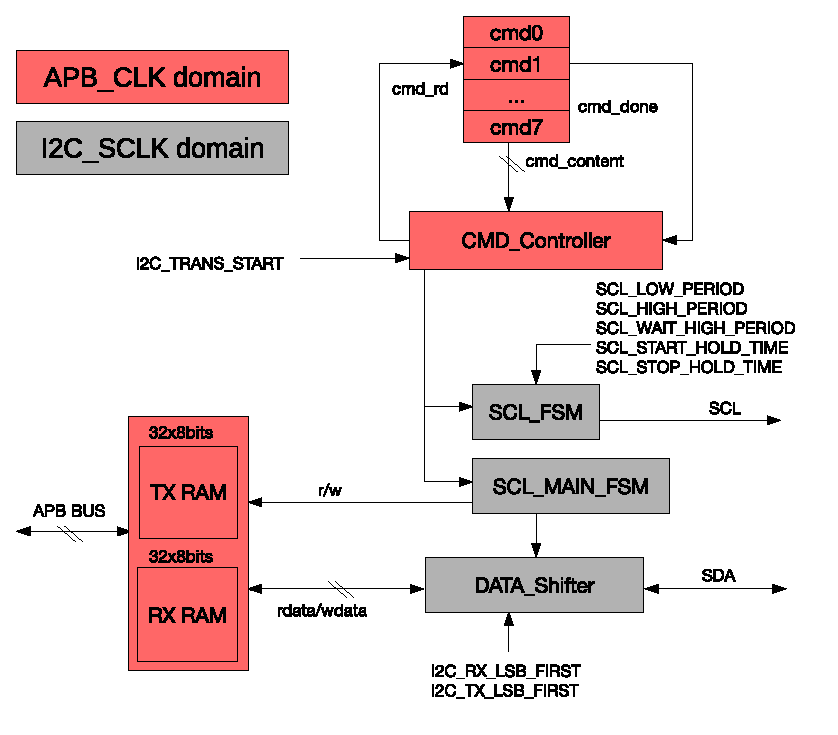
\includegraphics[width=0.65\textwidth]{\modulefiles/figures/728_i2c_master_architecture}
    \caption{I2C Master Architecture}
    \label{fig:i2c-master}
\end{figure}

\begin{figure}[H]
    \centering
    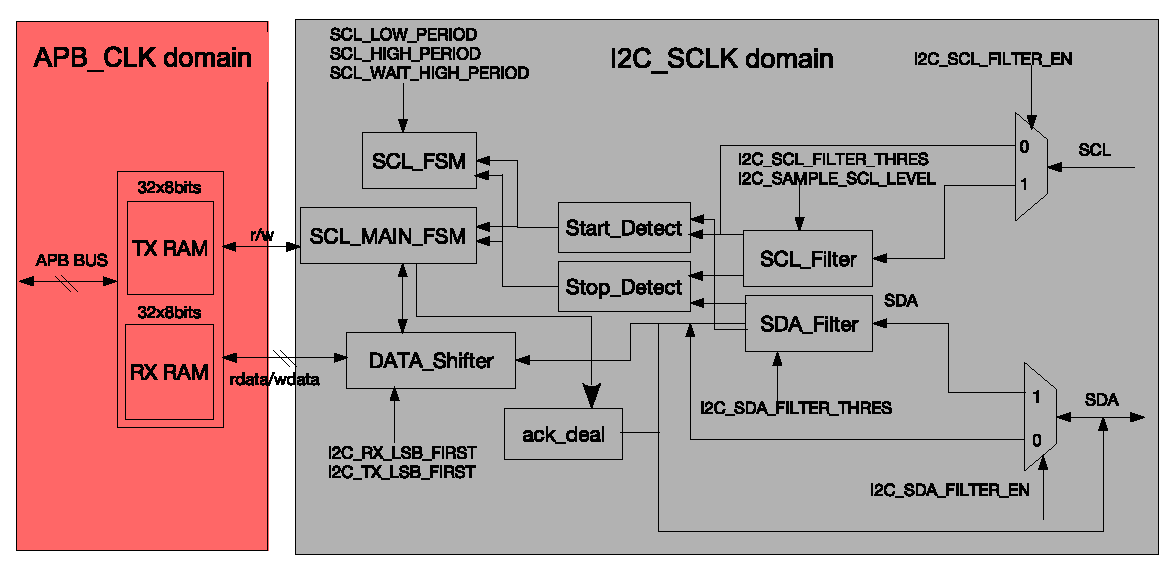
\includegraphics[width=0.8\textwidth]{\modulefiles/figures/728_i2c_slave_architecture}
    \caption{I2C Slave Architecture}
    \label{fig:i2c-slave}
\end{figure}

The I2C controller runs either in master mode or slave mode, which is determined by \hyperref[fielddesc:I2CMSMODE]{I2C\_MS\_MODE}. Figure \ref{fig:i2c-master} shows the architecture of a master, while Figure \ref{fig:i2c-slave} shows that of a slave. The I2C controller has the following main parts:
\begin{itemize}
    \item transmit and receive memory (TX/RX RAM)
    \item command controller (CMD\_Controller)
    \item SCL clock controller (SCL\_FSM)
    \item SDA data controller (SCL\_MAIN\_FSM)
    \item serial/parallel data converter (DATA\_Shifter)
    \item filter for SCL (SCL\_Filter)
    \item filter for SDA (SDA\_Filter)
\end{itemize}

Besides, the I2C controller also has a clock module which generates I2C clocks, and a synchronization module which synchronizes the APB bus and the I2C controller.

The clock module is used to select clock sources, turn on and off clocks, and divide clocks. SCL\_Filter and SDA\_Filter remove noises on SCL input signals and SDA input signals respectively. The synchronization module synchronizes signal transfer between different clock domains.

Figure \ref{fig:i2c-protocol-timing} and Figure \ref{fig:i2c-timing-param} are the timing diagram and corresponding parameters of the I2C protocol. SCL\_FSM generates the timing sequence conforming to the I2C protocol.

SCL\_MAIN\_FSM controls the execution of I2C commands and the sequence of the SDA line. CMD\_Controller is used for an I2C master to generate (R)START, STOP, WRITE, READ and END commands. TX RAM and RX RAM store data to be transmitted and data received respectively. DATA\_Shifter shifts data between serial and parallel form.


\begin{figure}[H]
    \centering
    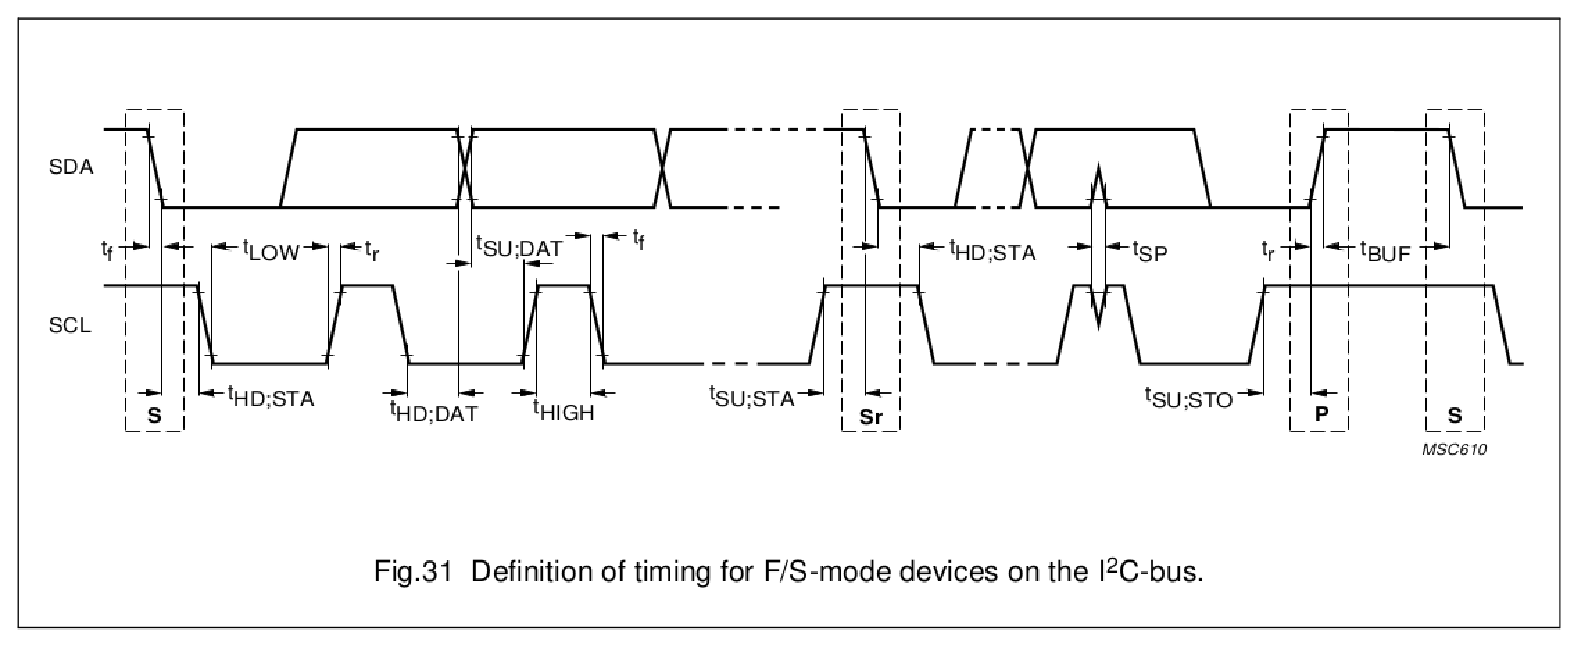
\includegraphics[width=0.9\textwidth]{\modulefiles/figures/i2c_timing_definition}
    \caption{I2C Protocol Timing (Cited from Fig.31 in \href{https://www.csd.uoc.gr/~hy428/reading/i2c_spec.pdf}{The I2C-bus specification} Version 2.1)}
    \label{fig:i2c-protocol-timing}
\end{figure}

\begin{figure}[H]
    \centering
    \fbox{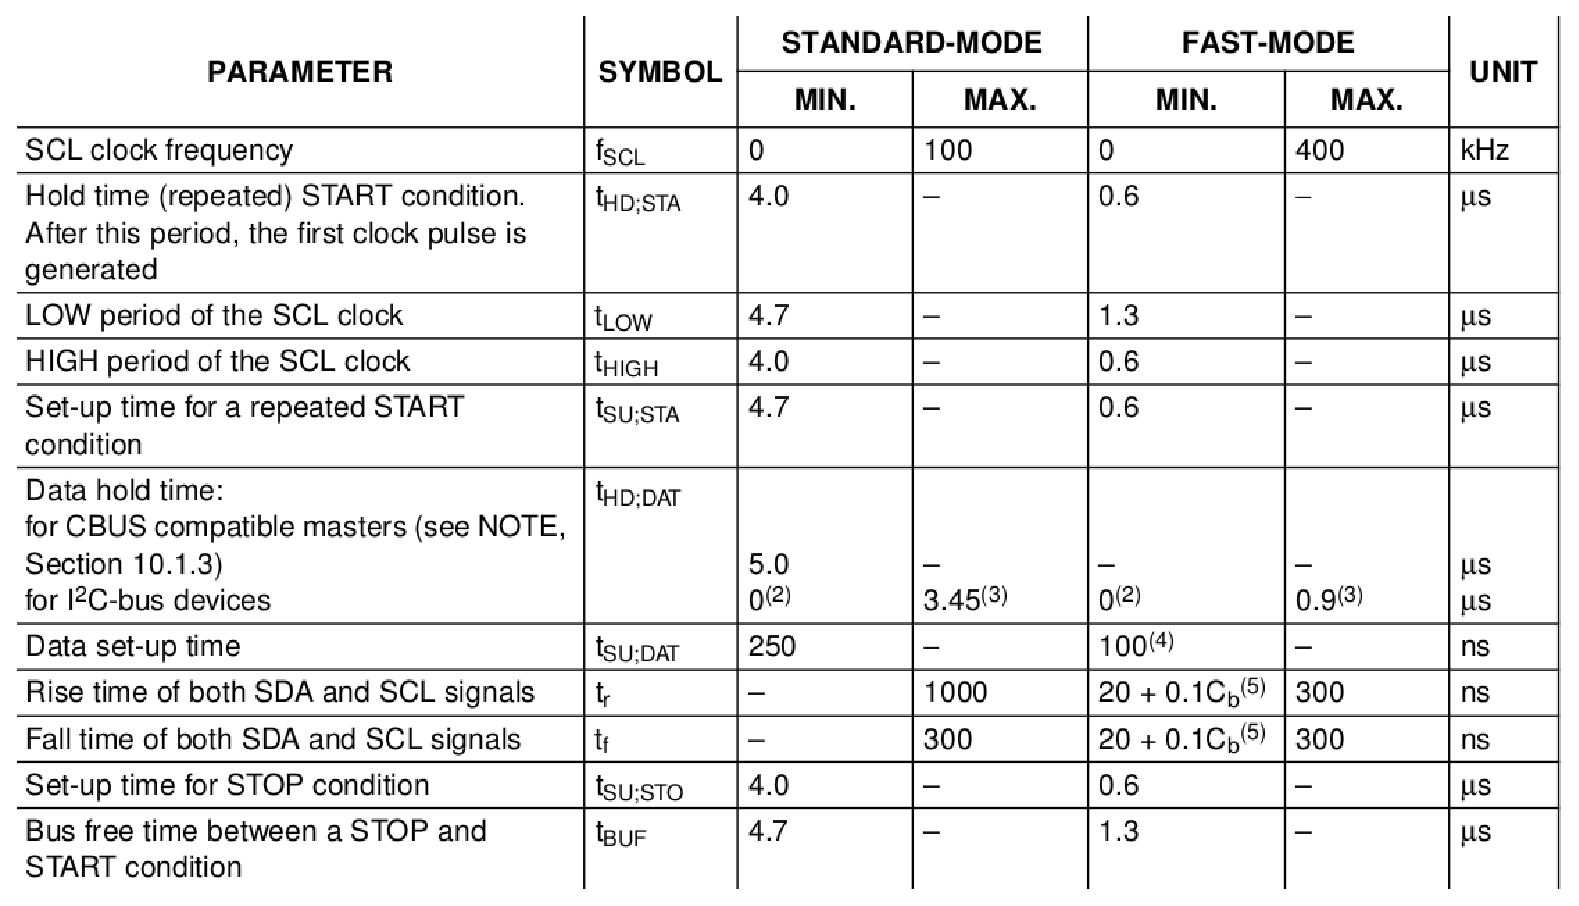
\includegraphics[width=0.9\textwidth]{\modulefiles/figures/i2c_timing_characteristic}}
    \caption{I2C Timing Parameters (Cited from Table 5 in \href{https://www.csd.uoc.gr/~hy428/reading/i2c_spec.pdf}{The I2C-bus specification} Version 2.1)}
    \label{fig:i2c-timing-param}
\end{figure}


\section{Functional Description}
Note that operations may differ between the I2C controller in \chipname{} and other masters or slaves on the bus. Please refer to datasheets of individual I2C devices for specific information.

\subsection{Clock Configuration}
Registers, TX RAM, and RX RAM are configured and accessed in the APB\_CLK clock domain, whose frequency is 1 $\sim$ 80 MHz. The main logic of the I2C controller, including SCL\_FSM, SCL\_MAIN\_FSM, SCL\_FILTER, SDA\_FILTER, and DATA\_SHIFTER, are in the I2C\_SCLK clock domain.

You can choose the clock source for I2C\_SCLK from XTAL\_CLK or RC\_FAST\_CLK via \hyperref[fielddesc:I2CSCLKSEL]{I2C\_SCLK\_SEL}. When \hyperref[fielddesc:I2CSCLKSEL]{I2C\_SCLK\_SEL} is cleared, the clock source is XTAL\_CLK. When \hyperref[fielddesc:I2CSCLKSEL]{I2C\_SCLK\_SEL} is set, the clock source is RC\_FAST\_CLK. The clock source is enabled by configuring \hyperref[fielddesc:I2CSCLKACTIVE]{I2C\_SCLK\_ACTIVE} as high level, and then passes through a fractional divider to generate I2C\_SCLK according to the following equation:

\[
Divisor = I2C\_SCLK\_DIV\_ NUM + 1+\frac{ \hyperref[fielddesc:I2CSCLKDIVA]{I2C\_SCLK\_DIV\_A}}{\hyperref[fielddesc:I2CSCLKDIVB]{I2C\_SCLK\_DIV\_B}}
\]

The frequency of XTAL\_CLK is 40 MHz, while the frequency of RC\_FAST\_CLK is 17.5 MHz. Limited by timing parameters, the derived clock I2C\_SCLK should operate at a frequency 20 timers larger than SCL's frequency.

\subsection{SCL and SDA Noise Filtering}
SCL\_Filter and SDA\_Filter modules are identical and are used to filter signal noises on SCL and SDA, respectively. These filters can be enabled or disabled by configuring \hyperref[fielddesc:I2CSCLFILTEREN]{I2C\_SCL\_FILTER\_EN} and \hyperref[fielddesc:I2CSDAFILTEREN]{I2C\_SDA\_FILTER\_EN}.

Take SCL\_Filter as an example. When enabled, SCL\_Filter samples input signals on the SCL line continuously. These input signals are valid only if they remain unchanged for consecutive \hyperref[fielddesc:I2CSCLFILTERTHRES]{I2C\_SCL\_FILTER\_THRES} I2C\_SCLK clock cycles. Given that only valid input signals can pass through the filter, SCL\_Filter can remove glitches whose pulse width is shorter than \hyperref[fielddesc:I2CSCLFILTERTHRES]{I2C\_SCL\_FILTER\_THRES} I2C\_SCLK clock cycles, while SDA\_Filter can remove glitches whose pulse width is shorter than \hyperref[fielddesc:I2CSDAFILTERTHRES]{I2C\_SDA\_FILTER\_THRES} I2C\_SCLK clock cycles.

\subsection{SCL Clock Stretching}
The I2C controller in slave mode (i.e. slave) can hold the SCL line low in exchange for more time to process data. This function called clock stretching is enabled by setting the \hyperref[fielddesc:I2CSLAVESCLSTRETCHEN]{I2C\_SLAVE\_SCL\_STRETCH\_EN} bit. The time period to release the SCL line from stretching is configured by setting the \hyperref[fielddesc:I2CSTRETCHPROTECTNUM]{I2C\_STRETCH\_PROTECT\_NUM} field, in order to avoid timing sequence errors.
The slave will hold the SCL line low when one of the following four events occurs:

\begin{enumerate}
\item Address match: The address of the slave matches the address sent by the master via the SDA line, and the $R/\overline W$ bit is 1.
\item RAM being full: RX RAM of the slave is full. Note that when the slave receives less than 32 bytes, it is not necessary to enable clock stretching; when the slave receives 32 bytes or more, you may interrupt data transmission to wrapped around RAM via the FIFO threshold, or enable clock stretching for more time to process data. When clock stretching is nabled, \hyperref[fielddesc:I2CRXFULLACKLEVEL]{I2C\_RX\_FULL\_ACK\_LEVEL} must be cleared, otherwise there will be unpredictable consequences.
\item RAM being empty: The slave is sending data, but its TX RAM is empty.
\item Sending an ACK: If \hyperref[fielddesc:I2CSLAVEBYTEACKCTLEN]{I2C\_SLAVE\_BYTE\_ACK\_CTL\_EN} is set, the slave pulls SCL low when sending an ACK bit. At this stage, software validates data and configures \hyperref[fielddesc:I2CSLAVEBYTEACKLVL]{I2C\_SLAVE\_BYTE\_ACK\_LVL} to control the level of the ACK bit. Note that when RX RAM of the slave is full, the level of the ACK bit to be sent is determined by \hyperref[fielddesc:I2CRXFULLACKLEVEL]{I2C\_RX\_FULL\_ACK\_LEVEL}, instead of \hyperref[fielddesc:I2CSLAVEBYTEACKLVL]{I2C\_SLAVE\_BYTE\_ACK\_LVL}. In this case, \hyperref[fielddesc:I2CRXFULLACKLEVEL]{I2C\_RX\_FULL\_ACK\_LEVEL} should also be cleared to ensure proper functioning of clock stretching.
\end{enumerate}

After SCL has been stretched low, the cause of stretching can be read from the \hyperref[fielddesc:I2CSTRETCHCAUSE]{I2C\_STRETCH\_CAUSE} bit. Clock stretching is disabled by setting the \hyperref[fielddesc:I2CSLAVESCLSTRETCHCLR]{I2C\_SLAVE\_SCL\_STRETCH\_CLR} bit.

\subsection{Generating SCL Pulses in Idle State}
Usually when the I2C bus is idle, the SCL line is held high. The I2C controller in \chipname{} can be programmed to generate SCL pulses in idle state. This function only works when the I2C controller is configured as master. If the \hyperref[fielddesc:I2CSCLRSTSLVEN]{I2C\_SCL\_RST\_SLV\_EN} bit is set, hardware will send \hyperref[fielddesc:I2CSCLRSTSLVNUM]{I2C\_SCL\_RST\_SLV\_NUM} SCL pulses, and then automatically clear this bit. When software reads 0 in  \hyperref[fielddesc:I2CSCLRSTSLVEN]{I2C\_SCL\_RST\_SLV\_EN}, set \hyperref[fielddesc:I2CCONFUPGATE]{I2C\_CONF\_UPGATE} to stop this function.

\subsection{Synchronization}
I2C registers are configured in APB\_CLK domain, whereas the I2C controller is configured in asynchronous I2C\_SCLK domain. Therefore, before being used by the I2C controller, register values should be synchronized by first writing configuration registers and then writing 1 to \hyperref[fielddesc:I2CCONFUPGATE]{I2C\_CONF\_UPGATE}. Registers that need synchronization are listed in Table \ref{tab:i2c-sync-register}.

\clearpage
\begin{longtable}{ | p{6cm} | p{7cm} | p{2cm} | }
\caption{I2C Synchronous Registers}
\label{tab:i2c-sync-register}
\\\hline
\rowcolor{lightgray}
Register & Parameter & Address  \\ \hline


\hyperref[regdesc:I2CCTRREG]{I2C\_CTR\_REG} & {\hyperref[fielddesc:I2CSLVTXAUTOSTARTEN]{I2C\_SLV\_TX\_AUTO\_START\_EN}} & 0x{}0004  \\\cline{2-2}

& {\hyperref[fielddesc:I2CADDR10BITRWCHECKEN]{I2C\_ADDR\_10BIT\_RW\_CHECK\_EN}}& \\\cline{2-2}
& {\hyperref[fielddesc:I2CADDRBROADCASTINGEN]{I2C\_ADDR\_BROADCASTING\_EN}}& \\\cline{2-2}
& {\hyperref[fielddesc:I2CSDAFORCEOUT]{I2C\_SDA\_FORCE\_OUT}}& \\\cline{2-2}
& {\hyperref[fielddesc:I2CSCLFORCEOUT]{I2C\_SCL\_FORCE\_OUT}}& \\\cline{2-2}
& {\hyperref[fielddesc:I2CSAMPLESCLLEVEL]{I2C\_SAMPLE\_SCL\_LEVEL}}& \\\cline{2-2}
& {\hyperref[fielddesc:I2CRXFULLACKLEVEL]{I2C\_RX\_FULL\_ACK\_LEVEL}}& \\\cline{2-2}
& {\hyperref[fielddesc:I2CMSMODE]{I2C\_MS\_MODE}}& \\\cline{2-2}
& {\hyperref[fielddesc:I2CTXLSBFIRST]{I2C\_TX\_LSB\_FIRST}}& \\\cline{2-2}
& {\hyperref[fielddesc:I2CRXLSBFIRST]{I2C\_RX\_LSB\_FIRST}}& \\\cline{2-2}
& {\hyperref[fielddesc:I2CARBITRATIONEN]{I2C\_ARBITRATION\_EN}}& \\ \hline

\hyperref[regdesc:I2CTOREG]{I2C\_TO\_REG} & {\hyperref[fielddesc:I2CTIMEOUTEN]{I2C\_TIME\_OUT\_EN}} & 0x{}000C  \\\cline{2-2}
& {\hyperref[fielddesc:I2CTIMEOUTVALUE]{I2C\_TIME\_OUT\_VALUE}}& \\ \hline

\hyperref[regdesc:I2CSLAVEADDRREG]{I2C\_SLAVE\_ADDR\_REG} & {\hyperref[fielddesc:I2CADDR10BITEN]{I2C\_ADDR\_10BIT\_EN}} & 0x{}0010 \\\cline{2-2}
& {\hyperref[fielddesc:I2CSLAVEADDR]{I2C\_SLAVE\_ADDR}}& \\ \hline


\hyperref[regdesc:I2CFIFOCONFREG]{I2C\_FIFO\_CONF\_REG} & {\hyperref[fielddesc:I2CFIFOADDRCFGEN]{I2C\_FIFO\_ADDR\_CFG\_EN}} & 0x{}0018 \\ \hline

\hyperref[regdesc:I2CSCLSPCONFREG]{I2C\_SCL\_SP\_CONF\_REG} & {\hyperref[fielddesc:I2CSDAPDEN]{I2C\_SDA\_PD\_EN}} & 0x{}0080  \\\cline{2-2}
& {\hyperref[fielddesc:I2CSCLPDEN]{I2C\_SCL\_PD\_EN}}& \\\cline{2-2}
& {\hyperref[fielddesc:I2CSCLRSTSLVNUM]{I2C\_SCL\_RST\_SLV\_NUM}}& \\\cline{2-2}
& {\hyperref[fielddesc:I2CSCLRSTSLVEN]{I2C\_SCL\_RST\_SLV\_EN}}& \\ \hline


\hyperref[regdesc:I2CSCLSTRETCHCONFREG]{I2C\_SCL\_STRETCH\_CONF\_REG} & {\hyperref[fielddesc:I2CSLAVEBYTEACKCTLEN]{I2C\_SLAVE\_BYTE\_ACK\_CTL\_EN}} & 0x{}0084  \\\cline{2-2}
& {\hyperref[fielddesc:I2CSLAVEBYTEACKLVL]{I2C\_SLAVE\_BYTE\_ACK\_LVL}}& \\\cline{2-2}
& {\hyperref[fielddesc:I2CSLAVESCLSTRETCHEN]{I2C\_SLAVE\_SCL\_STRETCH\_EN}}& \\\cline{2-2}
& {\hyperref[fielddesc:I2CSTRETCHPROTECTNUM]{I2C\_STRETCH\_PROTECT\_NUM}}& \\ \hline


\hyperref[regdesc:I2CSCLLOWPERIODREG]{I2C\_SCL\_LOW\_PERIOD\_REG} & \hyperref[fielddesc:I2CSCLLOWPERIOD]{I2C\_SCL\_LOW\_PERIOD} & 0x{}0000  \\ \hline

\hyperref[regdesc:I2CSCLHIGHPERIODREG]{I2C\_SCL\_HIGH\_PERIOD\_REG} & \hyperref[fielddesc:I2CSCLWAITHIGHPERIOD]{I2C\_WAIT\_HIGH\_PERIOD} & 0x{}0038  \\\cline{2-2}
& \hyperref[fielddesc:I2CSCLHIGHPERIOD]{I2C\_HIGH\_PERIOD}& \\ \hline

\hyperref[regdesc:I2CSDAHOLDREG]{I2C\_SDA\_HOLD\_REG} & \hyperref[fielddesc:I2CSDAHOLDTIME]{I2C\_SDA\_HOLD\_TIME} & 0x{}0030  \\\hline
\hyperref[regdesc:I2CSDASAMPLEREG]{I2C\_SDA\_SAMPLE\_REG} & \hyperref[fielddesc:I2CSDASAMPLETIME]{I2C\_SDA\_SAMPLE\_TIME} & 0x{}0034  \\ \hline

\hyperref[regdesc:I2CSCLSTARTHOLDREG]{I2C\_SCL\_START\_HOLD\_REG} & \hyperref[fielddesc:I2CSCLSTARTHOLDTIME]{I2C\_SCL\_START\_HOLD\_TIME} & 0x{}0040  \\ \hline
\hyperref[regdesc:I2CSCLRSTARTSETUPREG]{I2C\_SCL\_RSTART\_SETUP\_REG} & \hyperref[fielddesc:I2CSCLRSTARTSETUPTIME]{I2C\_SCL\_RSTART\_SETUP\_TIME} & 0x{}0044  \\ \hline

\hyperref[regdesc:I2CSCLSTOPHOLDREG]{I2C\_SCL\_STOP\_HOLD\_REG} & \hyperref[fielddesc:I2CSCLSTOPHOLDTIME]{I2C\_SCL\_STOP\_HOLD\_TIME} & 0x{}0048  \\ \hline
\hyperref[regdesc:I2CSCLSTOPSETUPREG]{I2C\_SCL\_STOP\_SETUP\_REG} & \hyperref[fielddesc:I2CSCLSTOPSETUPTIME]{I2C\_SCL\_STOP\_SETUP\_TIME} & 0x{}004C  \\ \hline

\hyperref[regdesc:I2CSCLSTTIMEOUTREG]{I2C\_SCL\_ST\_TIME\_OUT\_REG}& \hyperref[fielddesc:I2CSCLSTTOI2C]{I2C\_SCL\_ST\_TO\_I2C} & 0x{}0078\\ \hline
\hyperref[regdesc:I2CSCLMAINSTTIMEOUTREG] {\hyperref[regdesc:I2CSCLMAINSTTIMEOUTREG]{I2C\_SCL\_MAIN\_ST\_TIME\_OUT\_REG}}& \hyperref[fielddesc:I2CSCLMAINSTTOI2C]{I2C\_SCL\_MAIN\_ST\_TO\_I2C} & 0x{}007C\\ \hline


\hyperref[regdesc:I2CFILTERCFGREG]{I2C\_FILTER\_CFG\_REG} & {\hyperref[fielddesc:I2CSCLFILTEREN]{I2C\_SCL\_FILTER\_EN}} & 0x{}0050  \\\cline{2-2}
& {\hyperref[fielddesc:I2CSCLFILTERTHRES]{I2C\_SCL\_FILTER\_THRES}}& \\\cline{2-2}
& {\hyperref[fielddesc:I2CSDAFILTEREN]{I2C\_SDA\_FILTER\_EN}} &  \\\cline{2-2}
& {\hyperref[fielddesc:I2CSDAFILTERTHRES]{I2C\_SDA\_FILTER\_THRES}} & \\ \hline
\end{longtable}

\subsection{Open-Drain Output}
SCL and SDA output drivers must be configured as open drain. There are two ways to achieve this:
\begin{enumerate}
\item Set \hyperref[fielddesc:I2CSCLFORCEOUT]{I2C\_SCL\_FORCE\_OUT} and \hyperref[fielddesc:I2CSDAFORCEOUT]{I2C\_SDA\_FORCE\_OUT}, and configure \hyperref[fielddesc:GPIOPINNPADDRIVER]{GPIO\_PIN\regindex{n}\_PAD\_DRIVER} for corresponding SCL and SDA pads as open-drain.
\item Clear \hyperref[fielddesc:I2CSCLFORCEOUT]{I2C\_SCL\_FORCE\_OUT} and \hyperref[fielddesc:I2CSDAFORCEOUT]{I2C\_SDA\_FORCE\_OUT}.
\end{enumerate}

Because these lines are configured as open-drain, the low-to-high transition time of each line is longer, determined together by the pull-up resistor and line capacitance. The output duty cycle of I2C is limited by the SDA and SCL line's pull-up speed, mainly SCL's speed.

In addition, when \hyperref[fielddesc:I2CSCLFORCEOUT]{I2C\_SCL\_FORCE\_OUT} and \hyperref[fielddesc:I2CSCLPDEN]{I2C\_SCL\_PD\_EN} are set to 1, SCL can be forced low; when \hyperref[fielddesc:I2CSDAFORCEOUT]{I2C\_SDA\_FORCE\_OUT} and \hyperref[fielddesc:I2CSDAPDEN]{I2C\_SDA\_PD\_EN} are set to 1, SDA can be forced low.


\subsection{Timing Parameter Configuration}\label{subsec:i2c-timing-para}
\begin{figure}[H]
    \centering
    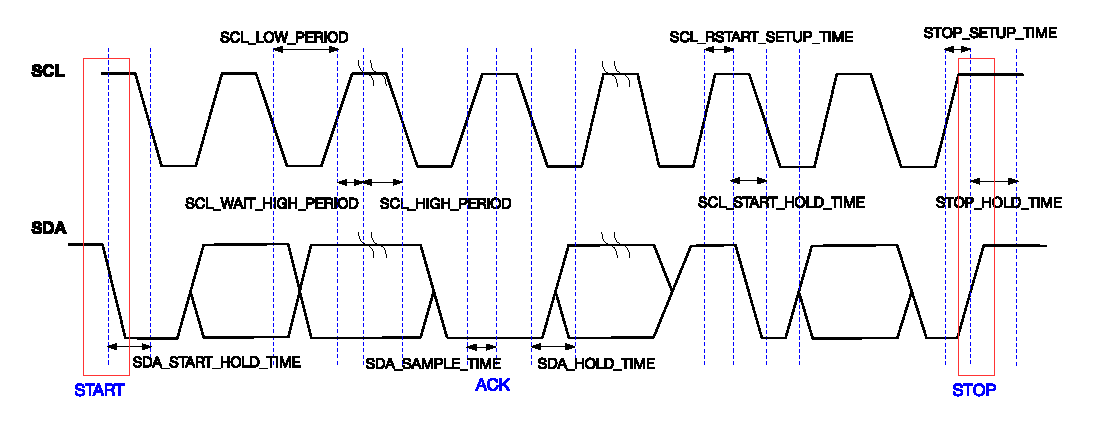
\includegraphics[width=0.9\textwidth]{\modulefiles/figures/I2C_bus_timing_723}
    \caption{I2C Timing Diagram}
    \label{fig:i2c-bus-timing}
\end{figure}

Figure \ref{fig:i2c-bus-timing} shows the timing diagram of an I2C master. This figure also specifies registers used to configure the START bit, STOP bit, data hold time, data sample time, waiting time on the rising SCL edge, etc. Timing parameters are calculated as follows in I2C\_SCLK clock cycles:

\begin{enumerate}
\item   $t_{LOW} = (\hyperref[fielddesc:I2CSCLLOWPERIOD]{I2C\_SCL\_LOW\_PERIOD} + 1) \cdot  T_{I2C\_SCLK}$

\item   $t_{HIGH} = (\hyperref[fielddesc:I2CSCLHIGHPERIOD]{I2C\_SCL\_HIGH\_PERIOD} + 1) \cdot  T_{I2C\_SCLK}$

\item   $t_{SU:STA} = (\hyperref[fielddesc:I2CSCLRSTARTSETUPTIME]{I2C\_SCL\_RSTART\_SETUP\_TIME} + 1) \cdot  T_{I2C\_SCLK}$

\item   $t_{HD:STA} = (\hyperref[fielddesc:I2CSCLSTARTHOLDTIME]{I2C\_SCL\_START\_HOLD\_TIME} +1) \cdot  T_{I2C\_SCLK}$

\item   $t_{r} = (\hyperref[fielddesc:I2CSCLWAITHIGHPERIOD]{I2C\_SCL\_WAIT\_HIGH\_PERIOD} + 1 ) \cdot  T_{I2C\_SCLK}$

\item   $t_{SU:STO} = (\hyperref[fielddesc:I2CSCLSTOPSETUPTIME]{I2C\_SCL\_STOP\_SETUP\_TIME}  + 1) \cdot  T_{I2C\_SCLK}$

\item   $t_{BUF} = (\hyperref[fielddesc:I2CSCLSTOPHOLDTIME]{I2C\_SCL\_STOP\_HOLD\_TIME}  + 1) \cdot  T_{I2C\_SCLK}$

\item   $t_{HD:DAT} = (\hyperref[fielddesc:I2CSDAHOLDTIME]{I2C\_SDA\_HOLD\_TIME} +1) \cdot  T_{I2C\_SCLK}$

\item   $t_{SU:DAT} = (\hyperref[fielddesc:I2CSCLLOWPERIOD]{I2C\_SCL\_LOW\_PERIOD} - \hyperref[fielddesc:I2CSDAHOLDTIME]{I2C\_SDA\_HOLD\_TIME}) \cdot  T_{I2C\_SCLK}$
\end{enumerate}

Timing registers below are divided into two groups, depending on the mode in which these registers are active:

\begin{itemize}
\item Master mode only:

\begin{enumerate}
\item \hyperref[fielddesc:I2CSCLSTARTHOLDTIME]{I2C\_SCL\_START\_HOLD\_TIME}:
Specifies the interval between pulling SDA low and pulling SCL low when the master generates a START condition. This interval is (\hyperref[fielddesc:I2CSCLSTARTHOLDTIME]{I2C\_SCL\_START\_HOLD\_TIME} +1) in I2C\_SCLK cycles. This register is active only when the I2C controller works in master mode.

\item \hyperref[fielddesc:I2CSCLLOWPERIOD]{I2C\_SCL\_LOW\_PERIOD}:
Specifies the low period of SCL. This period lasts (\hyperref[fielddesc:I2CSCLLOWPERIOD]{I2C\_SCL\_LOW\_PERIOD} +1) in I2C\_SCLK cycles. However, it could be extended when SCL is pulled low by peripheral devices or by an END command executed by the I2C controller, or when the clock is stretched. This register is active only when the I2C controller works in master mode.

\item \hyperref[fielddesc:I2CSCLWAITHIGHPERIOD]{I2C\_SCL\_WAIT\_HIGH\_PERIOD}:
Specifies time for SCL to go high in I2C\_SCLK cycles. Please make sure that SCL could be pulled high within this time period. Otherwise, the high period of SCL may be incorrect. This register is active only when the I2C controller works in master mode.

\item \hyperref[fielddesc:I2CSCLHIGHPERIOD]{I2C\_SCL\_HIGH\_PERIOD}:
Specifies the high period of SCL in I2C\_SCLK cycles. This register is active only when the I2C controller works in master mode.
When SCL goes high within (\hyperref[fielddesc:I2CSCLWAITHIGHPERIOD]{I2C\_SCL\_WAIT\_HIGH\_PERIOD} + 1) in I2C\_SCLK cycles, its frequency is:
\[
    f_{scl}=\frac{f_{\textrm{I2C\_SCLK}}}
    {\textrm{\hyperref[fielddesc:I2CSCLLOWPERIOD]{I2C\_SCL\_LOW\_PERIOD} + \hyperref[fielddesc:I2CSCLHIGHPERIOD]{I2C\_SCL\_HIGH\_PERIOD} + \hyperref[fielddesc:I2CSCLWAITHIGHPERIOD]{I2C\_SCL\_WAIT\_HIGH\_PERIOD}+3}}
\]
\end{enumerate}

\item Master mode and slave mode:

\begin{enumerate}
\item \hyperref[fielddesc:I2CSDASAMPLETIME]{I2C\_SDA\_SAMPLE\_TIME}:
Specifies the interval between the rising edge of SCL and the level sampling time of SDA. It is advised to set a value in the middle of SCL's high period, so as to correctly sample the level of SCL. This register is active both in master mode and slave mode.

\item \hyperref[fielddesc:I2CSDAHOLDTIME]{I2C\_SDA\_HOLD\_TIME}:
Specifies the interval between changing the SDA output level and the falling edge of SCL. This register is active both in master mode and slave mode.
\end{enumerate}

\end{itemize}

Timing parameters limits corresponding register configuration.
\begin{enumerate}
\item $\frac{f_{I2C\_SCLK}}{f_{SCL}}  > 20$
\item $3 \times f_{I2C\_SCLK} \leq (\hyperref[fielddesc:I2CSDAHOLDTIME]{I2C\_SDA\_HOLD\_TIME}-4) \times f_{APB\_CLK}$
\item \hyperref[fielddesc:I2CSDAHOLDTIME]{I2C\_SDA\_HOLD\_TIME} + \hyperref[fielddesc:I2CSCLSTARTHOLDTIME]{I2C\_SCL\_START\_HOLD\_TIME} > SDA\_FILTER\_THRES + 3
\item \hyperref[fielddesc:I2CSCLWAITHIGHPERIOD]{I2C\_SCL\_WAIT\_HIGH\_PERIOD} < \hyperref[fielddesc:I2CSDASAMPLETIME]{I2C\_SDA\_SAMPLE\_TIME} < \hyperref[fielddesc:I2CSCLHIGHPERIOD]{I2C\_SCL\_HIGH\_PERIOD}
\item \hyperref[fielddesc:I2CSDASAMPLETIME]{I2C\_SDA\_SAMPLE\_TIME} < \hyperref[fielddesc:I2CSCLWAITHIGHPERIOD]{I2C\_SCL\_WAIT\_HIGH\_PERIOD} + \hyperref[fielddesc:I2CSCLSTARTHOLDTIME]{I2C\_SCL\_START\_HOLD\_TIME} + \\\hyperref[fielddesc:I2CSCLRSTARTSETUPTIME]{I2C\_SCL\_RSTART\_SETUP\_TIME}
\item \hyperref[fielddesc:I2CSTRETCHPROTECTNUM]{I2C\_STRETCH\_PROTECT\_NUM} + \hyperref[fielddesc:I2CSDAHOLDTIME]{I2C\_SDA\_HOLD\_TIME} > \hyperref[fielddesc:I2CSCLLOWPERIOD]{I2C\_SCL\_LOW\_PERIOD}
\end{enumerate}

\subsection{Timeout Control}
The I2C controller has three types of timeout control, namely timeout control for SCL\_FSM, for SCL\_MAIN\_FSM, and for the SCL line. The first two are always enabled, while the third is configurable.

When SCL\_FSM remains unchanged for more than 2$^{\hyperref[fielddesc:I2CSCLSTTOI2C]{I2C\_SCL\_ST\_TO\_I2C}}$  clock cycles, an I2C\_SCL\_ST\_TO\_INT interrupt is triggered, and then SCL\_FSM goes to idle state. The value of \hyperref[fielddesc:I2CSCLSTTOI2C]{I2C\_SCL\_ST\_TO\_I2C} should be less than or equal to 22, which means SCL\_FSM could remain unchanged for 2$^{22}$ I2C\_SCLK clock cycles at most before the interrupt is generated.

When SCL\_MAIN\_FSM remains unchanged for more than 2$^{ \hyperref[fielddesc:I2CSCLMAINSTTOI2C]{I2C\_SCL\_MAIN\_ST\_TO\_I2C} }$ I2C\_SCLK clock cycles, an \\I2C\_SCL\_MAIN\_ST\_TO\_INT interrupt is triggered, and then SCL\_MAIN\_FSM goes to idle state. The value of \hyperref[fielddesc:I2CSCLMAINSTTOI2C]{I2C\_SCL\_MAIN\_ST\_TO\_I2C} should be less than or equal to 22, which means SCL\_MAIN\_FSM could remain unchanged for 2$^{22}$ clock cycles at most before the interrupt is generated.

Timeout control for SCL is enabled by setting \hyperref[fielddesc:I2CTIMEOUTEN]{I2C\_TIME\_OUT\_EN}. When the level of SCL remains unchanged for more than 2$^{\hyperref[fielddesc:I2CTIMEOUTVALUE]{I2C\_TIME\_OUT\_VALUE}}$ clock cycles, an I2C\_TIME\_OUT\_INT interrupt is triggered, and then the I2C bus goes to idle state.

\subsection{Command Configuration}\label{sec:i2c-func-descr-cmd-controller}
When the I2C controller works in master mode, CMD\_Controller reads commands from 8 sequential command registers and controls SCL\_FSM and SCL\_MAIN\_FSM accordingly.

\begin{figure}[H]
    \centering
    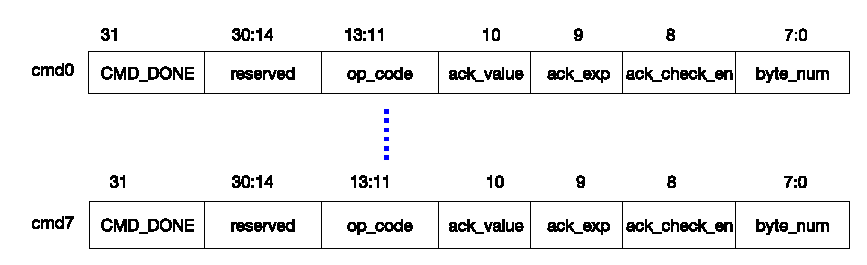
\includegraphics[width=0.8\textwidth]{\modulefiles/figures/I2C_Cmd_structure}
    \caption{Structure of I2C Command Registers}
    \label{fig:i2c-cmd-structure}
\end{figure}

Command registers, whose structure is illustrated in Figure \ref{fig:i2c-cmd-structure}, are active only when the I2C controller works in master mode. Fields of command registers are:

\begin{enumerate}

\item CMD\_DONE: Indicates that a command has been executed. After each command has been executed, the CMD\_DONE bit in the corresponding command register is set to 1 by hardware. By reading this bit, software can tell if the command has been executed. When writing new commands, this bit must be cleared by software.

\item op\_code: Indicates the command. The I2C controller supports five commands:

\begin{itemize}
    \item RSTART: op\_code = 6. The I2C controller sends a START bit or a RSTART bit defined by the I2C protocol.

    \item WRITE: op\_code = 1. The I2C controller sends a slave address, a register address  (only in double addressing mode) and data to the slave.

    \item READ: op\_code = 3. The I2C controller reads data from the slave.

    \item STOP: op\_code = 2. The I2C controller sends a STOP bit defined by the I2C protocol. This code also indicates that the command sequence has been executed, and the CMD\_Controller stops reading commands. After restarted by software, the CMD\_Controller resumes reading commands from command register 0.

    \item END: op\_code = 4. The I2C controller pulls the SCL line down and suspends I2C communication. This code also indicates that the command sequence has completed, and the CMD\_Controller stops executing commands. Once software refreshes data in command registers and the RAM, the CMD\_Controller can be restarted to execute commands from command register 0 again.
\end{itemize}

\item ack\_value: Used to configure the level of the ACK bit sent by the I2C controller during a read operation. This bit is ignored in RSTART, STOP, END and WRITE conditions.

\item ack\_exp: Used to configure the level of the ACK bit expected by the I2C controller during a write operation. This bit is ignored during RSTART, STOP, END and READ conditions.

\item ack\_check\_en: Used to enable the I2C controller during a write operation to check whether the ACK level sent by the slave matches ack\_exp in the command. If this bit is set and the level received does not match ack\_exp in the WRITE command, the master will generate an I2C\_NACK\_INT interrupt and a STOP condition for data transfer. If this bit is cleared, the controller will not check the ACK level sent by the slave. This bit is ignored during RSTART, STOP, END and READ conditions.

\item byte\_num: Specifies the length of data (in bytes) to be read or written. Can range from 1 to 255 bytes. This bit is ignored during RSTART, STOP and END conditions.
\end{enumerate}

Each command sequence is executed starting from command register 0 and terminated by a STOP or an END. Therefore, there must be a STOP or an END command in the eight command registers.

A complete data transfer on the I2C bus should be initiated by a START and terminated by a STOP. The transfer process may be completed using multiple sequences, separated by END commands. Each sequence may differ in the direction of data transfer, clock frequency, slave addresses, data length, etc. This allows efficient use of available peripheral RAM and also achieves more flexible I2C communication.

\subsection{TX/RX RAM Data Storage}\label{subsubsec:i2c-txrx}
Both TX RAM and RX RAM are 32 × 8 bits, and can be accessed in FIFO or non-FIFO mode. If \hyperref[fielddesc:I2CNONFIFOEN]{I2C\_NONFIFO\_EN} bit is cleared, both RAMs are accessed in FIFO mode; if \hyperref[fielddesc:I2CNONFIFOEN]{I2C\_NONFIFO\_EN} bit is set, both RAMs are accessed in non-FIFO mode.

TX RAM stores data that the I2C controller needs to send. During communication, when the I2C controller needs to send data (except acknowledgement bits), it reads data from TX RAM and sends them sequentially via SDA. When the I2C controller works in master mode, all data must be stored in TX RAM in the order they will be sent to slaves. The data stored in TX RAM include slave addresses, read/write bits, register addresses (only in double addressing mode) and data to be sent. When the I2C controller works in slave mode, TX RAM only stores data to be sent.

TX RAM can be read and written by the CPU. The CPU writes to TX RAM either in FIFO mode or in non-FIFO mode (direct address). In FIFO mode, the CPU writes to TX RAM via the fixed address \hyperref[regdesc:I2CDATAREG]{I2C\_DATA\_REG}, with addresses for writing in TX RAM incremented automatically by hardware. In non-FIFO mode, the CPU accesses TX RAM directly via address fields (\hyperref[tab:sysmem-base-address]{I2C Base Address} + 0x{}100) \textasciitilde (\hyperref[tab:sysmem-base-address]{I2C Base Address} + 0x{}17C). Each byte in TX RAM occupies an entire word in the address space. Therefore, the address of the first byte is \hyperref[tab:sysmem-base-address]{I2C Base Address} + 0x{}100, the second byte is \hyperref[tab:sysmem-base-address]{I2C Base Address} + 0x{}104, the third byte is \hyperref[tab:sysmem-base-address]{I2C Base Address} + 0x{}108, and so on. The CPU can only read TX RAM via direct addresses.
Addresses for reading TX RAM are the same with addresses for writing TX RAM.

RX RAM stores data the I2C controller receives during communication. When the I2C controller works in slave mode, neither slave addresses sent by the master nor register addresses (only in double addressing mode) will be stored into RX RAM. Values of RX RAM can be read by software after I2C communication completes.

RX RAM can only be read by the CPU. The CPU reads RX RAM either in FIFO mode or in non-FIFO mode (direct address). In FIFO mode, the CPU reads RX RAM via the fixed address \hyperref[regdesc:I2CDATAREG]{I2C\_DATA\_REG}, with addresses for reading RX RAM incremented automatically by hardware. In non-FIFO mode, the CPU accesses TX RAM directly via address fields (\hyperref[tab:sysmem-base-address]{I2C Base Address} + 0x{}180) \textasciitilde (\hyperref[tab:sysmem-base-address]{I2C Base Address} + 0x{}1FC). Each byte in RX RAM occupies an entire word in the address space. Therefore, the address of the first byte is \hyperref[tab:sysmem-base-address]{I2C Base Address} + 0x{}180, the second byte is \hyperref[tab:sysmem-base-address]{I2C Base Address} + 0x{}184, the third byte is \hyperref[tab:sysmem-base-address]{I2C Base Address} + 0x{}188 and so on.

In FIFO mode, TX RAM of a master may wrap around to send data larger than 32 bytes. Set \hyperref[fielddesc:I2CFIFOPRTEN]{I2C\_FIFO\_PRT\_EN}. If the size of data to be sent is smaller than \hyperref[fielddesc:I2CTXFIFOWMTHRHD]{I2C\_TXFIFO\_WM\_THRHD} (master), an I2C\_TXFIFO\_WM\_INT (master) interrupt is generated. After receiving the interrupt, software continues writing to \hyperref[regdesc:I2CDATAREG]{I2C\_DATA\_REG} (master). Please ensure that software writes to or refreshes TX RAM before the master sends data, otherwise it may result in unpredictable consequences.

In FIFO mode, RX RAM of a slave may also wrap around to receive data larger than 32 bytes. Set \hyperref[fielddesc:I2CFIFOPRTEN]{I2C\_FIFO\_PRT\_EN} and clear \hyperref[fielddesc:I2CRXFULLACKLEVEL]{I2C\_RX\_FULL\_ACK\_LEVEL}. If data already received (to be overwritten) is larger than \hyperref[fielddesc:I2CRXFIFOWMTHRHD]{I2C\_RXFIFO\_WM\_THRHD} (slave), an I2C\_RXFIFO\_WM\_INT (slave) interrupt is generated. After receiving the interrupt, software continues reading from \hyperref[regdesc:I2CDATAREG]{I2C\_DATA\_REG} (slave).

\subsection{Data Conversion}
DATA\_Shifter is used for serial/parallel conversion, converting byte data in TX RAM to an outgoing serial bitstream or an incoming serial bitstream to byte data in RX RAM. \hyperref[fielddesc:I2CRXLSBFIRST]{I2C\_RX\_LSB\_FIRST} and \hyperref[fielddesc:I2CTXLSBFIRST]{I2C\_TX\_LSB\_FIRST} can be used to select LSB- or MSB-first storage and transmission of data.

\subsection{Addressing Mode}
Besides 7-bit addressing, the \chipname{} I2C controller also supports 10-bit addressing and double addressing. 10-bit addressing can be mixed with 7-bit addressing.

Define the slave address as SLV\_ADDR. In 7-bit addressing mode, the slave address is SLV\_ADDR[6:0]; in 10-bit addressing mode, the slave address is SLV\_ADDR[9:0].

In 7-bit addressing mode, the master only needs to send one byte of address, which comprises SLV\_ADDR[6:0] and a $R/\overline W$ bit. In 7-bit addressing mode, there is a special case called general call addressing (broadcast). It is enabled by setting \hyperref[fielddesc:I2CADDRBROADCASTINGEN]{I2C\_ADDR\_BROADCASTING\_EN} in a slave. When the slave receives the general call address (0x{}00) from the master and the $R/\overline W$ bit followed is 0, it responds to the master regardless of its own address.

In 10-bit addressing mode, the master needs to send two bytes of address. The first byte is slave\_addr\_first\_7bits followed by a $R/\overline W$ bit, and slave\_addr\_first\_7bits should be configured as (0x{}78 | SLV\_ADDR[9:8]). The second byte is slave\_addr\_second\_byte, which should be configured as SLV\_ADDR[7:0]. The slave can enable 10-bit addressing by configuring \hyperref[fielddesc:I2CADDR10BITEN]{I2C\_ADDR\_10BIT\_EN}. \hyperref[fielddesc:I2CSLAVEADDR]{I2C\_SLAVE\_ADDR} is used to configure I2C slave address. Specifically, \hyperref[fielddesc:I2CSLAVEADDR]{I2C\_SLAVE\_ADDR}[14:7] should be configured as SLV\_ADDR[7:0], and  \hyperref[fielddesc:I2CSLAVEADDR]{I2C\_SLAVE\_ADDR}[6:0] should be configured as (0x{}78 | SLV\_ADDR[9:8]). Since a 10-bit slave address has one more byte than a 7-bit address, byte\_num of the WRITE command and the number of bytes in the RAM increase by one.

When working in slave mode, the I2C controller supports double addressing, where the first address is the address of an I2C slave, and the second one is the slave's memory address. When using double addressing, RAM must be accessed in non-FIFO mode. Double addressing is enabled by setting \hyperref[fielddesc:I2CFIFOADDRCFGEN]{I2C\_FIFO\_ADDR\_CFG\_EN}.

\subsection{\texorpdfstring{$R/\overline W$ Bit Check in 10-bit Addressing Mode}{R/W Bit Check in 10-bit Addressing Mode}}
In 10-bit addressing mode, when \hyperref[fielddesc:I2CADDR10BITRWCHECKEN]{I2C\_ADDR\_10BIT\_RW\_CHECK\_EN} is set to 1, the I2C controller performs a check on the first byte, which consists of slave\_addr\_first\_7bits and a $R/\overline W$ bit. When the $R/\overline W$ bit does not indicate a WRITE operation, i.e. not in line with the I2C protocol, the data transfer ends. If the check feature is not enabled, when the $R/\overline W$ bit does not indicate a WRITE, the data transfer still continues, but transfer failure may occur.

\subsection{To Start the I2C Controller}\label{subsubsec:i2c-start}
To start the I2C controller in master mode, after configuring the controller to master mode and command registers, write 1 to \hyperref[fielddesc:I2CTRANSSTART]{I2C\_TRANS\_START} in order that the master starts to parse and execute command sequences. The master always executes a command sequence starting from command register 0 to a STOP or an END at the end. To execute another command sequence starting from command register 0, refresh commands by writing 1 again to \hyperref[fielddesc:I2CTRANSSTART]{I2C\_TRANS\_START}.

To start the I2C controller in slave mode, there are two ways:

\begin{itemize}
    \item Set \hyperref[fielddesc:I2CSLVTXAUTOSTARTEN]{I2C\_SLV\_TX\_AUTO\_START\_EN}, and the slave starts automatic transfer upon an address match;
    \item Clear \hyperref[fielddesc:I2CSLVTXAUTOSTARTEN]{I2C\_SLV\_TX\_AUTO\_START\_EN}, and always set \hyperref[fielddesc:I2CTRANSSTART]{I2C\_TRANS\_START} before transfer.
\end{itemize}

\section{Programming Example}
This sections provides programming examples for typical communication scenarios. \chipname{} has one I2C controller. For the convenience of description, I2C masters and slaves in all subsequent figures are \chipname{} I2C controllers. I2C master is referred to as I2C$_\text{master}$, and I2C slave is referred to as I2C$_\text{slave}$.

\subsection{\texorpdfstring{I2C$_\text{master}$ Writes to I2C$_\text{slave}$ with a 7-bit Address in One Command Sequence}{I2C master Writes to I2C slave with a 7-bit Address in One Command Sequence}}\label{subsec:i2c-mws7}
\subsubsection{Introduction}
\begin{figure}[H]
    \centering
    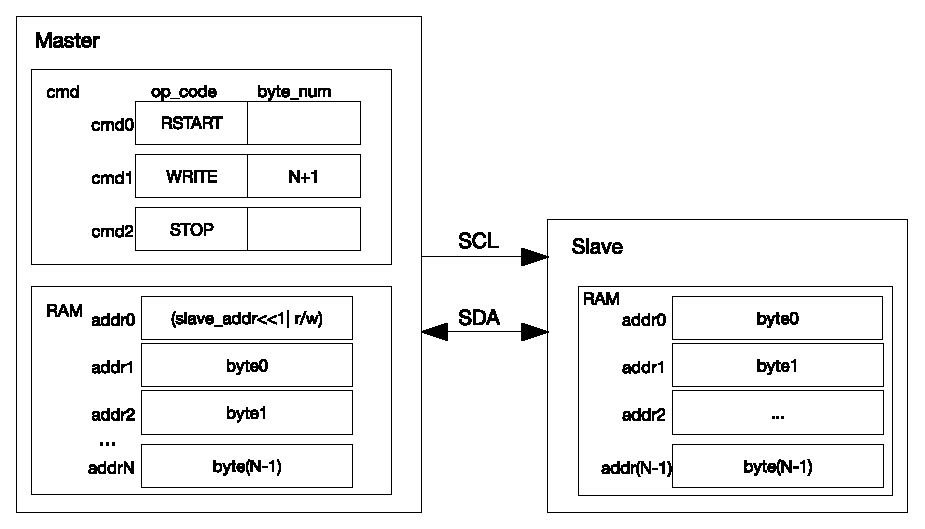
\includegraphics[width=0.8\textwidth]{\modulefiles/figures/I2C_MWS7}
    \caption{I2C$_\text{master}$ Writing to I2C$_\text{slave}$ with a 7-bit Address}
    \label{fig:i2c-mws7}
\end{figure}

Figure \ref{fig:i2c-mws7} shows how I2C$_\text{master}$ writes N bytes of data to I2C$_\text{slave}$ registers or RAM using 7-bit addressing. As shown in figure \ref{fig:i2c-mws7} , the first byte in the RAM of I2C$_\text{master}$ is a 7-bit I2C$_\text{slave}$ address followed by a $R/\overline W$ bit. When the $R/\overline W$ bit is 0, it indicates a WRITE operation. The remaining bytes are used to store data ready for transfer. The cmd box contains related command sequences.

After the command sequence is configured and data in RAM is ready, I2C$_\text{master}$ enables the controller and initiates data transfer by setting the \hyperref[fielddesc:I2CTRANSSTART]{I2C\_TRANS\_START} bit. The controller has four steps to take:
\begin{enumerate}
    \item Wait for SCL to go high, to avoid SCL being used by other masters or slaves.
    \item Execute a RSTART command and send a START bit.
    \item Execute a WRITE command by taking N+1 bytes from the RAM in order and send them to I2C$_\text{slave}$ in the same order. The first byte is the address of I2C$_\text{slave}$.
    \item Send a STOP. Once the I2C$_\text{master}$ transfers a STOP bit, an I2C\_TRANS\_COMPLETE\_INT interrupt is generated.
\end{enumerate}

\subsubsection{Configuration Example}
\begin{enumerate}
\item Configure the timing parameter registers of I2C$_\text{master}$ and I2C$_\text{slave}$ according to Section \ref{subsec:i2c-timing-para}.
\item Set \hyperref[fielddesc:I2CMSMODE]{I2C\_MS\_MODE} (master) to 1, and \hyperref[fielddesc:I2CMSMODE]{I2C\_MS\_MODE} (slave) to 0.
\item Write 1 to \hyperref[fielddesc:I2CCONFUPGATE]{I2C\_CONF\_UPGATE} (master) and \hyperref[fielddesc:I2CCONFUPGATE]{I2C\_CONF\_UPGATE} (slave) to synchronize registers.
\item Configure command registers of I2C$_\text{master}$.
\begin{longtable}{ | p{4cm} | p{2cm} | p{2cm} | p{2cm} |p{2cm} | p{2cm} |}
\hline\rowcolor{lightgray}
Command register& op\_code & ack\_value&ack\_exp&ack\_check\_en&byte\_num  \\ \hline
\hyperref[fielddesc:I2CCOMMAND0]{I2C\_COMMAND0} (master)& RSTART& ---&---&---&---  \\ \hline
\hyperref[fielddesc:I2CCOMMAND1]{I2C\_COMMAND1} (master)& WRITE& ack\_value&ack\_exp&1&N+1  \\ \hline
\hyperref[fielddesc:I2CCOMMAND2]{I2C\_COMMAND2} (master)& STOP& ---&---&---&---  \\ \hline
\end{longtable}
\item Write the address of I2C$_\text{slave}$ and data to be sent to TX RAM of I2C$_\text{master}$ in either FIFO mode or non-FIFO mode according to Section \ref{subsubsec:i2c-txrx}.
\item Write the address of I2C$_\text{slave}$ to \hyperref[fielddesc:I2CSLAVEADDR]{I2C\_SLAVE\_ADDR} (slave) in \hyperref[regdesc:I2CSLAVEADDRREG]{I2C\_SLAVE\_ADDR\_REG} (slave) register.
\item Write 1 to \hyperref[fielddesc:I2CCONFUPGATE]{I2C\_CONF\_UPGATE} (master) and \hyperref[fielddesc:I2CCONFUPGATE]{I2C\_CONF\_UPGATE} (slave) to synchronize registers.
\item Write 1 to \hyperref[fielddesc:I2CTRANSSTART]{I2C\_TRANS\_START} (master) and \hyperref[fielddesc:I2CTRANSSTART]{I2C\_TRANS\_START} (slave) to start transfer.
\item I2C$_\text{slave}$ compares the slave address sent by I2C$_\text{master}$ with its own address in \hyperref[fielddesc:I2CSLAVEADDR]{I2C\_SLAVE\_ADDR} (slave). When ack\_check\_en (master) in I2C$_\text{master}$'s WRITE command is 1, I2C$_\text{master}$ checks ACK value each time it sends a byte. When ack\_check\_en (master) is 0, I2C$_\text{master}$ does not check ACK value and take I2C$_\text{slave}$ as a matching slave by default.
\begin{itemize}
\item Match: If the received ACK value matches ack\_exp (master) (the expected ACK value), I2C$_\text{master}$ continues data transfer.
\item Not match: If the received ACK value does not match ack\_exp, I2C$_\text{master}$ generates an I2C\_NACK\_INT (master) interrupt and stops data transfer.
\end{itemize}

\item I2C$_\text{master}$ sends data, and checks ACK value or not according to ack\_check\_en (master).
\item If data to be sent (N) is larger than 32 bytes, TX RAM of I2C$_\text{master}$ may wrap around in FIFO mode. For details, please refer to Section \ref{subsubsec:i2c-txrx}.
\item If data to be received (N) is larger than 32 bytes, RX RAM of I2C$_\text{slave}$ may wrap around in FIFO mode. For details, please refer to Section \ref{subsubsec:i2c-txrx}.

If data to be received (N) is larger than 32 bytes, the other way is to enable clock stretching by setting the \hyperref[fielddesc:I2CSLAVESCLSTRETCHEN]{I2C\_SLAVE\_SCL\_STRETCH\_EN} (slave), and clearing \hyperref[fielddesc:I2CRXFULLACKLEVEL]{I2C\_RX\_FULL\_ACK\_LEVEL}. When RX RAM is full, an \hyperref[int:i2c-slave-stretch]{I2C\_SLAVE\_STRETCH\_INT} (slave) interrupt is generated. In this way, I2C$_\text{slave}$ can hold SCL low, in exchange for more time to read data. After software has finished reading, you can set \hyperref[fielddesc:I2CSLAVESTRETCHINTCLR]{I2C\_SLAVE\_STRETCH\_INT\_CLR} (slave) to 1 to clear interrupt, and set \hyperref[fielddesc:I2CSLAVESCLSTRETCHCLR]{I2C\_SLAVE\_SCL\_STRETCH\_CLR} (slave) to release the SCL line.

\item After data transfer completes, I2C$_\text{master}$ executes the STOP command, and generates an I2C\_TRANS\_COMPLETE\_INT (master) interrupt.

\end{enumerate}

\subsection{\texorpdfstring{I2C$_\text{master}$ Writes to I2C$_\text{slave}$ with a 10-bit Address in One Command Sequence}{I2C master Writes to I2C slave with a 10-bit Address in One Command Sequence}}\label{sub:i2c-app-mws10}
\subsubsection{Introduction}
\begin{figure}[H]
    \centering
    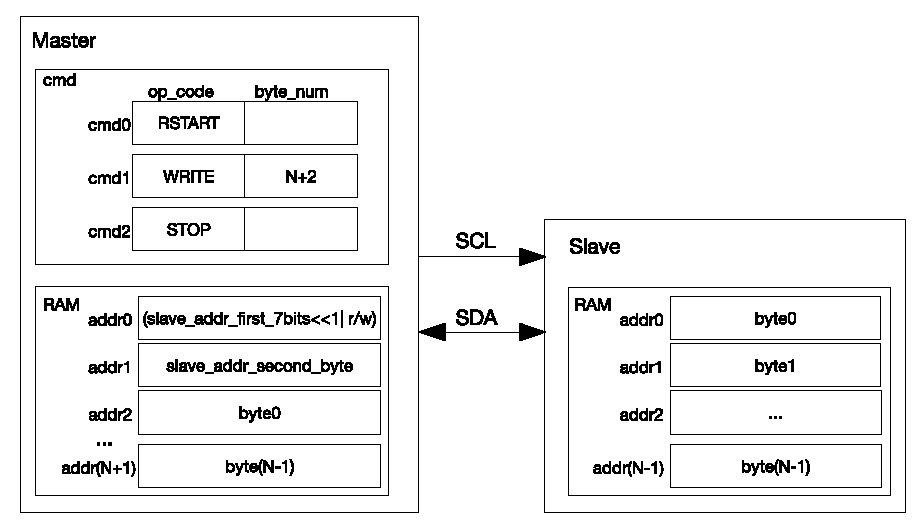
\includegraphics[width=0.8\textwidth]{\modulefiles/figures/I2C_MWS10}
    \caption{I2C$_\text{master}$ Writing to a Slave with a 10-bit Address}
    \label{fig:i2c-mws10}
\end{figure}

Figure \ref{fig:i2c-mws10} shows how I2C$_\text{master}$ writes N bytes of data using 10-bit addressing to an I2C slave. The configuration and transfer process is similar to what is described in \ref{subsec:i2c-mws7}, except that a 10-bit I2C$_\text{slave}$ address is formed from two bytes. Since a 10-bit I2C$_\text{slave}$ address has one more byte than a 7-bit I2C$_\text{slave}$ address, byte\_num and length of data in TX RAM increase by 1 accordingly.

\subsubsection{Configuration Example}
\begin{enumerate}
\item Set \hyperref[fielddesc:I2CMSMODE]{I2C\_MS\_MODE} (master) to 1, and \hyperref[fielddesc:I2CMSMODE]{I2C\_MS\_MODE} (slave) to 0.
\item Write 1 to \hyperref[fielddesc:I2CCONFUPGATE]{I2C\_CONF\_UPGATE} (master) and \hyperref[fielddesc:I2CCONFUPGATE]{I2C\_CONF\_UPGATE} (slave) to synchronize registers.
\item Configure command registers of I2C$_\text{master}$.

\begin{longtable}{ | p{4cm} | p{2cm} | p{2cm} | p{2cm} |p{2cm} | p{2cm} |}
\hline\rowcolor{lightgray}
Command registers& op\_code & ack\_value&ack\_exp&ack\_check\_en&byte\_num  \\ \hline
\hyperref[fielddesc:I2CCOMMAND0]{I2C\_COMMAND0} (master)& RSTART& ---&---&---&---  \\ \hline
\hyperref[fielddesc:I2CCOMMAND1]{I2C\_COMMAND1} (master)& WRITE& ack\_value&ack\_exp&1&N+2  \\ \hline
\hyperref[fielddesc:I2CCOMMAND2]{I2C\_COMMAND2} (master)& STOP& ---&---&---&---  \\ \hline
\end{longtable}

\item Configure \hyperref[fielddesc:I2CSLAVEADDR]{I2C\_SLAVE\_ADDR} (slave) in \hyperref[regdesc:I2CSLAVEADDRREG]{I2C\_SLAVE\_ADDR\_REG} (slave) as I2C$_\text{slave}$'s 10-bit address, and set \hyperref[fielddesc:I2CADDR10BITEN]{I2C\_ADDR\_10BIT\_EN} (slave) to 1 to enable 10-bit addressing.
\item Write the address of I2C$_\text{slave}$ and data to be sent to TX RAM of I2C$_\text{master}$. The first byte of the address of I2C$_\text{slave}$ comprises ((0x{}78 | \hyperref[fielddesc:I2CSLAVEADDR]{I2C\_SLAVE\_ADDR}[9:8])<<1) and a $R/\overline W$ bit. The second byte of the address of I2C$_\text{slave}$ is \hyperref[fielddesc:I2CSLAVEADDR]{I2C\_SLAVE\_ADDR}[7:0]. These two bytes are followed by data to be sent in FIFO or non-FIFO mode.
\item Write 1 to \hyperref[fielddesc:I2CCONFUPGATE]{I2C\_CONF\_UPGATE} (master) and \hyperref[fielddesc:I2CCONFUPGATE]{I2C\_CONF\_UPGATE} (slave) to synchronize registers.
\item Write 1 to \hyperref[fielddesc:I2CTRANSSTART]{I2C\_TRANS\_START} (master) and \hyperref[fielddesc:I2CTRANSSTART]{I2C\_TRANS\_START} (slave) to start transfer.
\item I2C$_\text{slave}$ compares the slave address sent by I2C$_\text{master}$ with its own address in \hyperref[fielddesc:I2CSLAVEADDR]{I2C\_SLAVE\_ADDR} (slave). When ack\_check\_en (master) in I2C$_\text{master}$'s WRITE command is 1, I2C$_\text{master}$ checks ACK value each time it sends a byte. When ack\_check\_en (master) is 0, I2C$_\text{master}$ does not check ACK value and take I2C$_\text{slave}$ as matching slave by default.
\begin{itemize}
\item Match: If the received ACK value matches ack\_exp (master) (the expected ACK value), I2C$_\text{master}$ continues data transfer.
\item Not match: If the received ACK value does not match ack\_exp, I2C$_\text{master}$ generates an I2C\_NACK\_INT (master) interrupt and stops data transfer.
\end{itemize}

\item I2C$_\text{master}$ sends data, and checks ACK value or not according to ack\_check\_en (master).
\item If data to be sent is larger than 32 bytes, TX RAM of I2C$_\text{master}$ may wrap around in FIFO mode. For details, please refer to Section \ref{subsubsec:i2c-txrx}.
\item If data to be received is larger than 32 bytes, RX RAM of I2C$_\text{slave}$ may wrap around in FIFO mode. For details, please refer to Section \ref{subsubsec:i2c-txrx}.

If data to be received is larger than 32 bytes, the other way is to enable clock stretching by setting \hyperref[fielddesc:I2CSLAVESCLSTRETCHEN]{I2C\_SLAVE\_SCL\_STRETCH\_EN} (slave), and clearing \hyperref[fielddesc:I2CRXFULLACKLEVEL]{I2C\_RX\_FULL\_ACK\_LEVEL} to 0. When RX RAM is full, an \hyperref[int:i2c-slave-stretch]{I2C\_SLAVE\_STRETCH\_INT} (slave) interrupt is generated. In this way, I2C$_\text{slave}$ can hold SCL low, in exchange for more time to read data. After software has finished reading, you can set \hyperref[fielddesc:I2CSLAVESTRETCHINTCLR]{I2C\_SLAVE\_STRETCH\_INT\_CLR} (slave) to 1 to clear interrupt, and set \hyperref[fielddesc:I2CSLAVESCLSTRETCHCLR]{I2C\_SLAVE\_SCL\_STRETCH\_CLR} (slave) to release the SCL line.

\item After data transfer completes, I2C$_\text{master}$ executes the STOP command, and generates an I2C\_TRANS\_COMPLETE\_INT (master) interrupt.

\end{enumerate}



\subsection{\texorpdfstring{I2C$_\text{master}$ Writes to I2C$_\text{slave}$ with Two 7-bit Addresses in One Command Sequence}{I2C master Writes to I2C slave with Two 7-bit Addresses in One Command Sequence}}
\subsubsection{Introduction}
\begin{figure}[H]
    \centering
    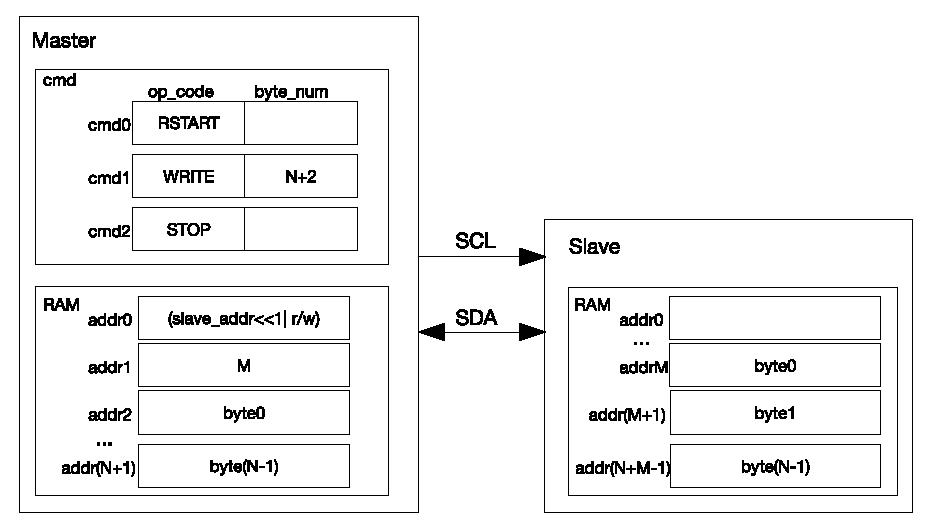
\includegraphics[width=0.8\textwidth]{\modulefiles/figures/I2C_MWS7_M}
    \caption{I2C$_\text{master}$ Writing to I2C$_\text{slave}$ with Two 7-bit Addresses}
    \label{fig:i2c-mws7-double}
\end{figure}

Figure \ref{fig:i2c-mws7-double} shows how I2C$_\text{master}$ writes N bytes of data to I2C$_\text{slave}$ registers or RAM using 7-bit double addressing. The configuration and transfer process is similar to what is described in Section \ref{subsec:i2c-mws7}, except that in 7-bit double addressing mode I2C$_\text{master}$ sends two 7-bit addresses. The first address is the address of an I2C slave, and the second one is I2C$_\text{slave}$'s memory address (i.e. addrM in Figure \ref{fig:i2c-mws7-double}). When using double addressing, RAM must be accessed in non-FIFO mode.
The I2C slave put received byte0 \verb+~+ byte(N-1) into its RAM in an order staring from addrM. The RAM is overwritten every 32 bytes.

\subsubsection{Configuration Example}
\begin{enumerate}
\item Set \hyperref[fielddesc:I2CMSMODE]{I2C\_MS\_MODE} (master) to 1, and \hyperref[fielddesc:I2CMSMODE]{I2C\_MS\_MODE} (slave) to 0.
\item Set \hyperref[fielddesc:I2CFIFOADDRCFGEN]{I2C\_FIFO\_ADDR\_CFG\_EN} (slave) to 1 to enable double addressing mode.
\item Write 1 to \hyperref[fielddesc:I2CCONFUPGATE]{I2C\_CONF\_UPGATE} (master) and \hyperref[fielddesc:I2CCONFUPGATE]{I2C\_CONF\_UPGATE} (slave) to synchronize registers.
\item Configure command registers of I2C$_\text{master}$.
\begin{longtable}{ | p{4cm} | p{2cm} | p{2cm} | p{2cm} |p{2cm} | p{2cm} |}
\hline\rowcolor{lightgray}
Command registers& op\_code & ack\_value&ack\_exp&ack\_check\_en&byte\_num  \\ \hline
\hyperref[fielddesc:I2CCOMMAND0]{I2C\_COMMAND0} (master)& RSTART& ---&---&---&---  \\ \hline
\hyperref[fielddesc:I2CCOMMAND1]{I2C\_COMMAND1} (master)& WRITE& ack\_value&ack\_exp&1&N+2  \\ \hline
\hyperref[fielddesc:I2CCOMMAND2]{I2C\_COMMAND2} (master)& STOP& ---&---&---&---  \\ \hline
\end{longtable}
\item Write the address of I2C$_\text{slave}$ and data to be sent to TX RAM of I2C$_\text{master}$ in FIFO or non-FIFO mode.
\item Write the address of I2C$_\text{slave}$ to \hyperref[fielddesc:I2CSLAVEADDR]{I2C\_SLAVE\_ADDR} (slave) in \hyperref[regdesc:I2CSLAVEADDRREG]{I2C\_SLAVE\_ADDR\_REG} (slave) register.
\item Write 1 to \hyperref[fielddesc:I2CCONFUPGATE]{I2C\_CONF\_UPGATE} (master) and \hyperref[fielddesc:I2CCONFUPGATE]{I2C\_CONF\_UPGATE} (slave) to synchronize registers.
\item Write 1 to \hyperref[fielddesc:I2CTRANSSTART]{I2C\_TRANS\_START} (master) and \hyperref[fielddesc:I2CTRANSSTART]{I2C\_TRANS\_START} (slave) to start transfer.
\item I2C$_\text{slave}$ compares the slave address sent by I2C$_\text{master}$ with its own address in \hyperref[fielddesc:I2CSLAVEADDR]{I2C\_SLAVE\_ADDR} (slave). When ack\_check\_en (master) in I2C$_\text{master}$'s WRITE command is 1, I2C$_\text{master}$ checks ACK value each time it sends a byte. When ack\_check\_en (master) is 0, I2C$_\text{master}$ does not check ACK value and take I2C$_\text{slave}$ as matching slave by default.
\begin{itemize}
\item Match: If the received ACK value matches ack\_exp (master) (the expected ACK value), I2C$_\text{master}$ continues data transfer.
\item Not match: If the received ACK value does not match ack\_exp, I2C$_\text{master}$ generates an I2C\_NACK\_INT (master) interrupt and stops data transfer.
\end{itemize}
\item I2C$_\text{slave}$ receives the RX RAM address sent by I2C$_\text{master}$ and adds the offset.

\item I2C$_\text{master}$ sends data, and checks ACK value or not according to ack\_check\_en (master).
\item If data to be sent is larger than 32 bytes, TX RAM of I2C$_\text{master}$ may wrap around in FIFO mode. For details, please refer to Section \ref{subsubsec:i2c-txrx}.
\item If data to be received is larger than 32 bytes, you may enable clock stretching by setting \hyperref[fielddesc:I2CSLAVESCLSTRETCHEN]{I2C\_SLAVE\_SCL\_STRETCH\_EN} (slave), and clearing \hyperref[fielddesc:I2CRXFULLACKLEVEL]{I2C\_RX\_FULL\_ACK\_LEVEL} to 0. When RX RAM is full, an \hyperref[int:i2c-slave-stretch]{I2C\_SLAVE\_STRETCH\_INT} (slave) interrupt is generated. In this way, I2C$_\text{slave}$ can hold SCL low, in exchange for more time to read data. After software has finished reading, you can set \hyperref[fielddesc:I2CSLAVESTRETCHINTCLR]{I2C\_SLAVE\_STRETCH\_INT\_CLR} (slave) to 1 to clear interrupt, and set \hyperref[fielddesc:I2CSLAVESCLSTRETCHCLR]{I2C\_SLAVE\_SCL\_STRETCH\_CLR} (slave) to release the SCL line.
\item After data transfer completes, I2C$_\text{master}$ executes the STOP command, and generates an I2C\_TRANS\_COMPLETE\_INT (master) interrupt.

\end{enumerate}

\subsection{\texorpdfstring{I2C$_\text{master}$ Writes to I2C$_\text{slave}$ with a 7-bit Address in Multiple Command Sequences}{I2C master Writes to I2C slave with a 7-bit Address in Multiple Command Sequences}}
\subsubsection{Introduction}
\begin{figure}[H]
    \centering
    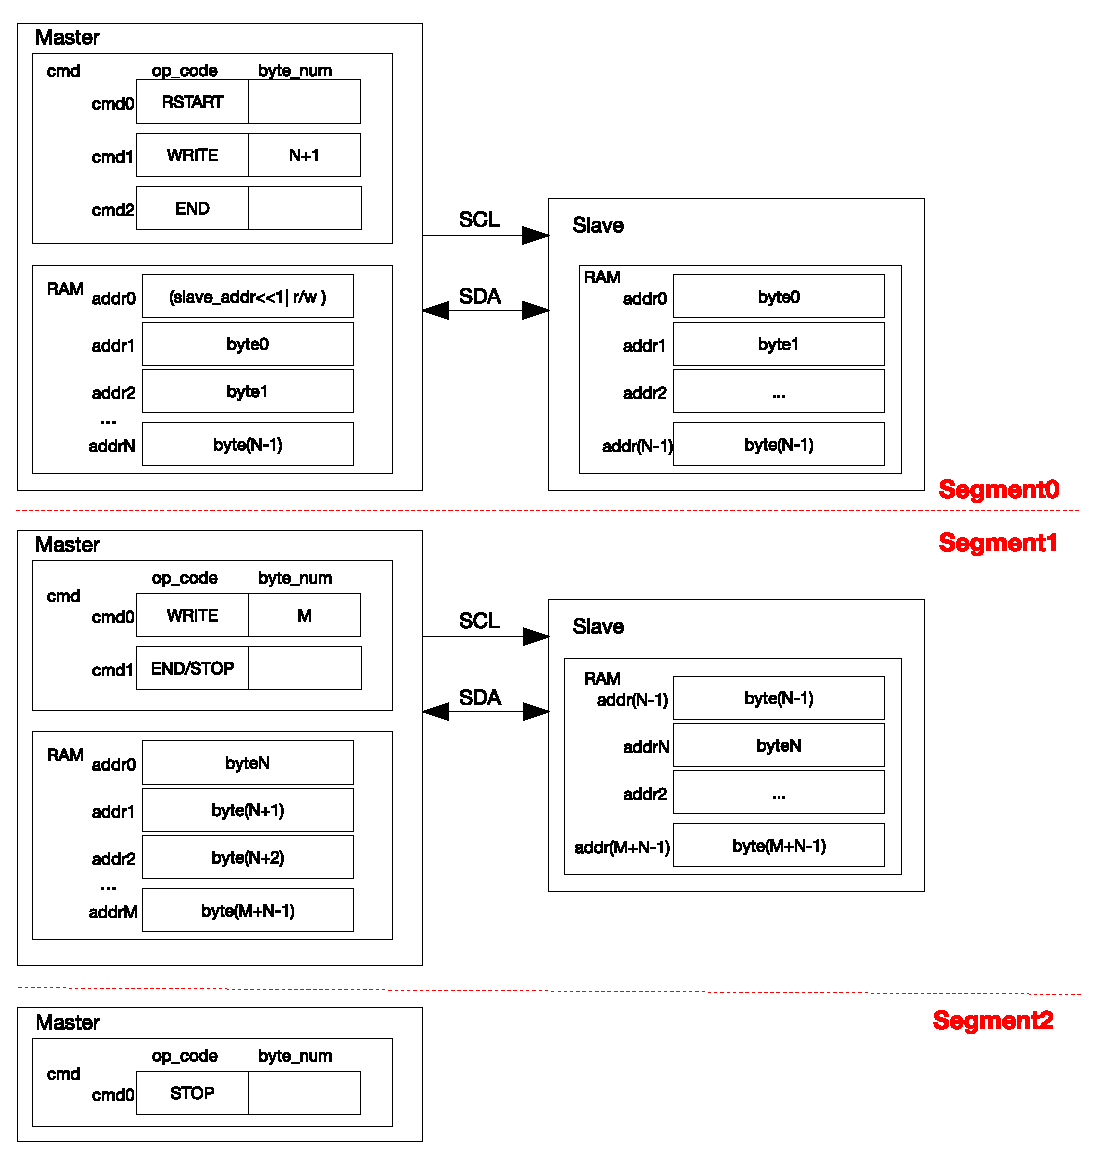
\includegraphics[width=0.8\textwidth]{\modulefiles/figures/I2C_MWS_END}    \caption{I2C$_\text{master}$ Writing to I2C$_\text{slave}$ with a 7-bit Address in Multiple Sequences}
    \label{fig:i2c-mws7-multiple}
\end{figure}

Given that the I2C Controller RAM holds only 32 bytes, when data are too large to be processed even by the wrapped RAM, it is advised to transmit them in multiple command sequences. At the end of every command sequence is an END command. When the controller executes this END command to pull SCL low, software refreshes command sequence registers and the RAM for next the transfer.

Figure \ref{fig:i2c-mws7-multiple} shows how I2C$_\text{master}$ writes to an I2C slave in two or three segments as an example. For the first segment, the CMD\_Controller registers are configured as shown in Segment0. Once data in I2C$_\text{master}$'s RAM is ready and \hyperref[fielddesc:I2CTRANSSTART]{I2C\_TRANS\_START} is set, I2C$_\text{master}$ initiates data transfer. After executing the END command, I2C$_\text{master}$ turns off the SCL clock and pulls SCL low to reserve the bus. Meanwhile, the controller generates an I2C\_END\_DETECT\_INT interrupt.

For the second segment, after detecting the I2C\_END\_DETECT\_INT interrupt, software refreshes the CMD\_Controller registers, reloads the RAM and clears this interrupt, as shown in Segment1. If cmd1 in the second segment is a STOP, then data is transmitted to I2C$_\text{slave}$ in two segments. I2C$_\text{master}$ resumes data transfer after \hyperref[fielddesc:I2CTRANSSTART]{I2C\_TRANS\_START} is set, and terminates the transfer by sending a STOP bit.

For the third segment, after the second data transfer finishes and an I2C\_END\_DETECT\_INT is detected, the CMD\_Controller registers of I2C$_\text{master}$ are configured as shown in Segment2. Once \hyperref[fielddesc:I2CTRANSSTART]{I2C\_TRANS\_START} is set, I2C$_\text{master}$ generates a STOP bit and terminates the transfer.

Note that other I2C$_\text{master}$s will not transact on the bus between two segments. The bus is only released after a STOP signal is sent. The I2C controller can be reset by setting \hyperref[fielddesc:I2CFSMRST]{I2C\_FSM\_RST} field at any time. This field will later be cleared automatically by hardware.

\subsubsection{Configuration Example}
\begin{enumerate}
\item Set \hyperref[fielddesc:I2CMSMODE]{I2C\_MS\_MODE} (master) to 1, and \hyperref[fielddesc:I2CMSMODE]{I2C\_MS\_MODE} (slave) to 0.
\item Write 1 to \hyperref[fielddesc:I2CCONFUPGATE]{I2C\_CONF\_UPGATE} (master) and \hyperref[fielddesc:I2CCONFUPGATE]{I2C\_CONF\_UPGATE} (slave) to synchronize registers.
\item Configure command registers of I2C$_\text{master}$.
\begin{longtable}{ | p{4cm} | p{2cm} | p{2cm} | p{2cm} |p{2cm} | p{2cm} |}
\hline\rowcolor{lightgray}
Command registers& op\_code & ack\_value&ack\_exp&ack\_check\_en&byte\_num  \\ \hline
\hyperref[fielddesc:I2CCOMMAND0]{I2C\_COMMAND0} (master)& RSTART& ---&---&---&---  \\ \hline
\hyperref[fielddesc:I2CCOMMAND1]{I2C\_COMMAND1} (master)& WRITE& ack\_value&ack\_exp&1&N+1  \\ \hline
\hyperref[fielddesc:I2CCOMMAND2]{I2C\_COMMAND2} (master)& END& ---&---&---&---  \\ \hline
\end{longtable}
\item Write the address of I2C$_\text{slave}$ and data to be sent to TX RAM of I2C$_\text{master}$ in either FIFO mode or non-FIFO mode according to Section \ref{subsubsec:i2c-txrx}.
\item Write the address of I2C$_\text{slave}$ to \hyperref[fielddesc:I2CSLAVEADDR]{I2C\_SLAVE\_ADDR} (slave) in \hyperref[regdesc:I2CSLAVEADDRREG]{I2C\_SLAVE\_ADDR\_REG} (slave) register
\item Write 1 to \hyperref[fielddesc:I2CCONFUPGATE]{I2C\_CONF\_UPGATE} (master) and \hyperref[fielddesc:I2CCONFUPGATE]{I2C\_CONF\_UPGATE} (slave) to synchronize registers.
\item Write 1 to \hyperref[fielddesc:I2CTRANSSTART]{I2C\_TRANS\_START} (master) and \hyperref[fielddesc:I2CTRANSSTART]{I2C\_TRANS\_START} (slave) to start transfer.
\item I2C$_\text{slave}$ compares the slave address sent by I2C$_\text{master}$ with its own address in \hyperref[fielddesc:I2CSLAVEADDR]{I2C\_SLAVE\_ADDR} (slave). When ack\_check\_en (master) in I2C$_\text{master}$'s WRITE command is 1, I2C$_\text{master}$ checks ACK value each time it sends a byte. When ack\_check\_en (master) is 0, I2C$_\text{master}$ does not check ACK value and take I2C$_\text{slave}$ as matching slave by default.
\begin{itemize}
\item Match: If the received ACK value matches ack\_exp (master) (the expected ACK value), I2C$_\text{master}$ continues data transfer.
\item Not match: If the received ACK value does not match ack\_exp, I2C$_\text{master}$ generates an I2C\_NACK\_INT (master) interrupt and stops data transfer.
\end{itemize}

\item I2C$_\text{master}$ sends data, and checks ACK value or not according to ack\_check\_en (master).

\item After the I2C\_END\_DETECT\_INT (master) interrupt is generated, set \hyperref[fielddesc:I2CENDDETECTINTCLR]{I2C\_END\_DETECT\_INT\_CLR} (master) to 1 to clear this interrupt.
\item Update I2C$_\text{master}$'s command registers.
\begin{longtable}{ | p{4cm} | p{2cm} | p{2cm} | p{2cm} |p{2cm} | p{2cm} |}
\hline\rowcolor{lightgray}
Command registers& op\_code & ack\_value&ack\_exp&ack\_check\_en&byte\_num  \\ \hline
\hyperref[fielddesc:I2CCOMMAND0]{I2C\_COMMAND0} (master)& WRITE& ack\_value&ack\_exp&1&M  \\ \hline
\hyperref[fielddesc:I2CCOMMAND1]{I2C\_COMMAND1} (master)& END/STOP& ---&---&---&---  \\ \hline
\end{longtable}
\item Write M bytes of data to be sent to TX RAM of I2C$_\text{master}$ in FIFO or non-FIFO mode.
\item Write 1 to \hyperref[fielddesc:I2CTRANSSTART]{I2C\_TRANS\_START} (master) bit to start transfer and repeat step 9.
\item If the command is a STOP, I2C stops transfer and generates an I2C\_TRANS\_COMPLETE\_INT (master) interrupt.
\item If the command is an END, repeat step 10.
\item Update I2C$_\text{master}$'s command registers.
\begin{longtable}{ | p{4cm} | p{2cm} | p{2cm} | p{2cm} |p{2cm} | p{2cm} |}
\hline\rowcolor{lightgray}
Command registers of I2C$_\text{master}$& op\_code & ack\_value&ack\_exp&ack\_check\_en&byte\_num  \\ \hline
\hyperref[fielddesc:I2CCOMMAND1]{I2C\_COMMAND1} (master)& STOP& ---&---&---&---  \\ \hline
\end{longtable}
\item Write 1 to \hyperref[fielddesc:I2CTRANSSTART]{I2C\_TRANS\_START} (master) bit to start transfer.
\item I2C$_\text{master}$ executes the STOP command and generates an I2C\_TRANS\_COMPLETE\_INT (master) interrupt.

\end{enumerate}

\subsection{\texorpdfstring{I2C$_\text{master}$ Reads I2C$_\text{slave}$ with a 7-bit Address in One Command Sequence}{I2C master Reads I2C slave with a 7-bit Address in One Command Sequence}}
\subsubsection{Introduction}
\begin{figure}[H]
    \centering
    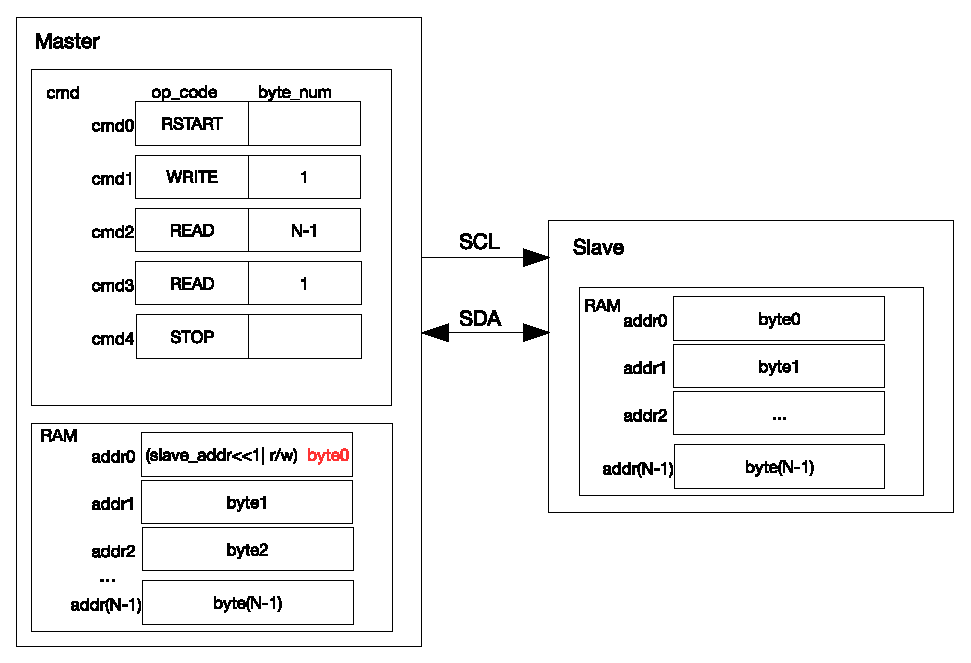
\includegraphics[width=0.8\textwidth]{\modulefiles/figures/I2C_MRS7}
    \caption{I2C$_\text{master}$ Reading I2C$_\text{slave}$ with a 7-bit Address}
    \label{fig:i2c-mrs7}
\end{figure}

Figure \ref{fig:i2c-mrs7} shows how I2C$_\text{master}$ reads N bytes of data from an I2C slave using 7-bit addressing. cmd1 is a WRITE command, and when this command is executed I2C$_\text{master}$ sends the address of I2C$_\text{slave}$. The byte sent comprises a 7-bit I2C$_\text{slave}$ address and a $R/\overline W$ bit. When the $R/\overline W$ bit is 1, it indicates a READ operation. If the address of an I2C slave matches the sent address, this matching slave starts sending data to I2C$_\text{master}$. I2C$_\text{master}$ generates acknowledgements according to ack\_value defined in the READ command upon receiving a byte.

As illustrated in Figure \ref{fig:i2c-mrs7}, I2C$_\text{master}$ executes two READ commands: it generates ACKs for (N-1) bytes of data in cmd2, and a NACK for the last byte of data in cmd 3. This configuration may be changed as required. I2C$_\text{master}$ writes received data into the controller RAM from addr0, whose original content (a the address of I2C$_\text{slave}$ and a $R/\overline W$ bit) is overwritten by byte0 marked red in Figure \ref{fig:i2c-mrs7}.

\subsubsection{Configuration Example}
\begin{enumerate}
\item Set \hyperref[fielddesc:I2CMSMODE]{I2C\_MS\_MODE} (master) to 1, and \hyperref[fielddesc:I2CMSMODE]{I2C\_MS\_MODE} (slave) to 0.
\item We recommend setting \hyperref[fielddesc:I2CSLAVESCLSTRETCHEN]{I2C\_SLAVE\_SCL\_STRETCH\_EN} (slave) to 1, so that SCL can be held low for more processing time when I2C$_\text{slave}$ needs to send data. If this bit is not set, software should write data to be sent to I2C$_\text{slave}$'s TX RAM before I2C$_\text{master}$ initiates transfer. Configuration below is applicable to scenario where \hyperref[fielddesc:I2CSLAVESCLSTRETCHEN]{I2C\_SLAVE\_SCL\_STRETCH\_EN} (slave) is 1.
\item Write 1 to \hyperref[fielddesc:I2CCONFUPGATE]{I2C\_CONF\_UPGATE} (master) and \hyperref[fielddesc:I2CCONFUPGATE]{I2C\_CONF\_UPGATE} (slave) to synchronize registers.
\item Configure command registers of I2C$_\text{master}$.
\begin{longtable}{ | p{4cm} | p{2cm} | p{2cm} | p{2cm} |p{2cm} | p{2cm} |}
\hline\rowcolor{lightgray}
Command registers of I2C$_\text{master}$& op\_code & ack\_value&ack\_exp&ack\_check\_en&byte\_num  \\ \hline
\hyperref[fielddesc:I2CCOMMAND0]{I2C\_COMMAND0} (master)& RSTART& ---&---&---&---  \\ \hline
\hyperref[fielddesc:I2CCOMMAND1]{I2C\_COMMAND1} (master)& WRITE& 0&0&1&1  \\ \hline
\hyperref[fielddesc:I2CCOMMAND2]{I2C\_COMMAND2} (master)& READ& 0&0&1&N-1  \\ \hline
\hyperref[fielddesc:I2CCOMMAND3]{I2C\_COMMAND3} (master)& READ& 1&0&1&1  \\ \hline
\hyperref[fielddesc:I2CCOMMAND4]{I2C\_COMMAND4} (master)& STOP& ---&---&---&---  \\ \hline
\end{longtable}
\item Write the address of I2C$_\text{slave}$ to TX RAM of I2C$_\text{master}$ in either FIFO mode or non-FIFO mode according to Section \ref{subsubsec:i2c-txrx}.
\item Write the address of I2C$_\text{slave}$ to \hyperref[fielddesc:I2CSLAVEADDR]{I2C\_SLAVE\_ADDR} (slave) in \hyperref[regdesc:I2CSLAVEADDRREG]{I2C\_SLAVE\_ADDR\_REG} (slave) register.
\item Write 1 to \hyperref[fielddesc:I2CCONFUPGATE]{I2C\_CONF\_UPGATE} (master) and \hyperref[fielddesc:I2CCONFUPGATE]{I2C\_CONF\_UPGATE} (slave) to synchronize registers.
\item Write 1 to \hyperref[fielddesc:I2CTRANSSTART]{I2C\_TRANS\_START} (master) bit to start I2C$_\text{master}$'s transfer.
\item Start I2C$_\text{slave}$'s transfer according to Section \ref{subsubsec:i2c-start}.
\item I2C$_\text{slave}$ compares the slave address sent by I2C$_\text{master}$ with its own address in \hyperref[fielddesc:I2CSLAVEADDR]{I2C\_SLAVE\_ADDR} (slave). When ack\_check\_en (master) in I2C$_\text{master}$'s WRITE command is 1, I2C$_\text{master}$ checks ACK value each time it sends a byte. When ack\_check\_en (master) is 0, I2C$_\text{master}$ does not check ACK value and take I2C$_\text{slave}$ as matching slave by default.
\begin{itemize}
\item Match: If the received ACK value matches ack\_exp (master) (the expected ACK value), I2C$_\text{master}$ continues data transfer.
\item Not match: If the received ACK value does not match ack\_exp, I2C$_\text{master}$ generates an I2C\_NACK\_INT (master) interrupt and stops data transfer.
\end{itemize}

\item After \hyperref[int:i2c-slave-stretch]{I2C\_SLAVE\_STRETCH\_INT} (slave) is generated, the \hyperref[fielddesc:I2CSTRETCHCAUSE]{I2C\_STRETCH\_CAUSE} bit is 0. The address of I2C$_\text{slave}$ matches the address sent over SDA, and I2C$_\text{slave}$ needs to send data.
\item Write data to be sent to TX RAM of I2C$_\text{slave}$ in either FIFO mode or non-FIFO mode according to Section \ref{subsubsec:i2c-txrx}.
\item Set \hyperref[fielddesc:I2CSLAVESCLSTRETCHCLR]{I2C\_SLAVE\_SCL\_STRETCH\_CLR} (slave) to 1 to release SCL.

\item I2C$_\text{slave}$ sends data, and I2C$_\text{master}$ checks ACK value or not according to ack\_check\_en (master) in the READ command.

\item If data to be read by I2C$_\text{master}$ is larger than 32 bytes, an \hyperref[int:i2c-slave-stretch]{I2C\_SLAVE\_STRETCH\_INT} (slave) interrupt will be generated when TX RAM of I2C$_\text{slave}$ becomes empty. In this way, I2C$_\text{slave}$ can hold SCL low, so that software has more time to pad data in TX RAM of I2C$_\text{slave}$ and read data in RX RAM of I2C$_\text{master}$. After software has finished reading, you can set \hyperref[fielddesc:I2CSLAVESTRETCHINTCLR]{I2C\_SLAVE\_STRETCH\_INT\_CLR} (slave) to 1 to clear interrupt, and set \hyperref[fielddesc:I2CSLAVESCLSTRETCHCLR]{I2C\_SLAVE\_SCL\_STRETCH\_CLR} (slave) to release the SCL line.

\item After I2C$_\text{master}$ has received the last byte of data, set ack\_value (master) to 1. I2C$_\text{slave}$ will stop transfer once receiving the I2C\_NACK\_INT interrupt.

\item After data transfer completes, I2C$_\text{master}$ executes the STOP command, and generates an I2C\_TRANS\_COMPLETE\_INT (master) interrupt.

\end{enumerate}

\subsection{\texorpdfstring{I2C$_\text{master}$ Reads I2C$_\text{slave}$ with a 10-bit Address in One Command Sequence}{I2C master Reads I2C slave with a 10-bit Address in One Command Sequence}}
\subsubsection{Introduction}
\begin{figure}[H]
    \centering
    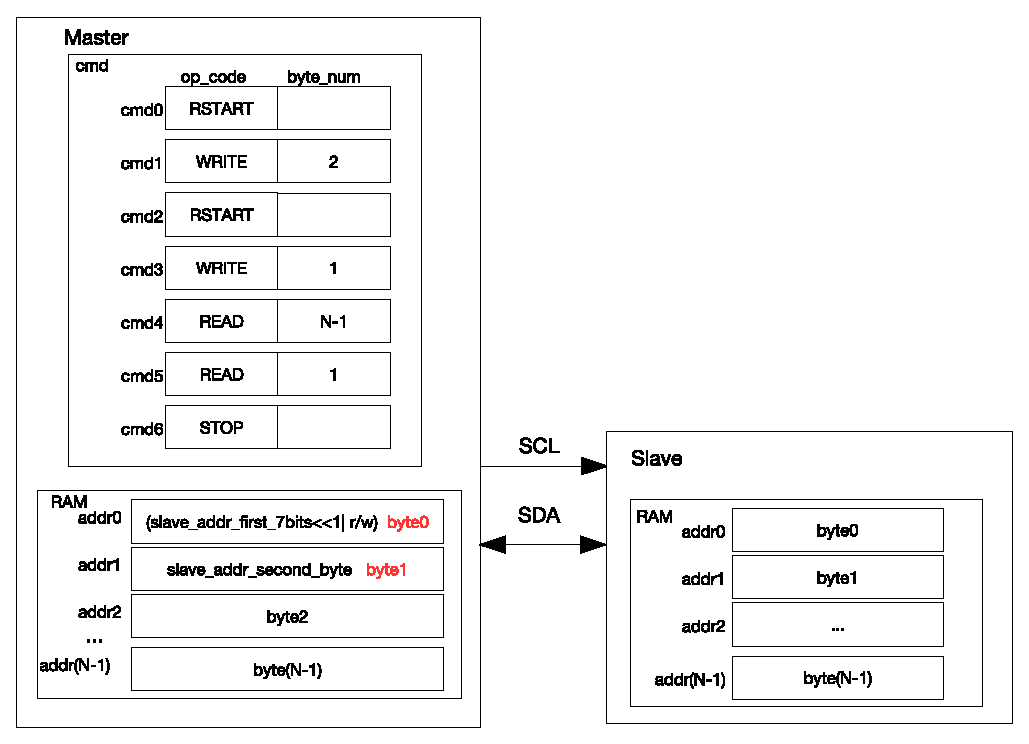
\includegraphics[width=0.8\textwidth]{\modulefiles/figures/I2C_MRS10}
    \caption{I2C$_\text{master}$ Reading I2C$_\text{slave}$ with a 10-bit Address}
    \label{fig:i2c-mrs10}
\end{figure}

Figure \ref{fig:i2c-mrs10} shows how I2C$_\text{master}$ reads data from an I2C slave using 10-bit addressing. Unlike 7-bit addressing, in 10-bit addressing the WRITE command of the I2C$_\text{master}$ is formed from two bytes, and correspondingly TX RAM of this master stores a 10-bit address of two bytes. The $R/\overline W$ bit in the first byte is 0, which indicates a WRITE operation. After a RSTART condition, I2C$_\text{master}$ sends the first byte of address again to read data from I2C$_\text{slave}$, but the $R/\overline W$ bit is 1, which indicates a READ operation. The two address bytes can be configured as described in Section \ref{sub:i2c-app-mws10}.

\subsubsection{Configuration Example}
\begin{enumerate}
\item Set \hyperref[fielddesc:I2CMSMODE]{I2C\_MS\_MODE} (master) to 1, and \hyperref[fielddesc:I2CMSMODE]{I2C\_MS\_MODE} (slave) to 0.
\item We recommend setting \hyperref[fielddesc:I2CSLAVESCLSTRETCHEN]{I2C\_SLAVE\_SCL\_STRETCH\_EN} (slave) to 1, so that SCL can be held low for more processing time when I2C$_\text{slave}$ needs to send data. If this bit is not set, software should write data to be sent to I2C$_\text{slave}$'s TX RAM before I2C$_\text{master}$ initiates transfer. Configuration below is applicable to scenario where \hyperref[fielddesc:I2CSLAVESCLSTRETCHEN]{I2C\_SLAVE\_SCL\_STRETCH\_EN} (slave) is 1.
\item Write 1 to \hyperref[fielddesc:I2CCONFUPGATE]{I2C\_CONF\_UPGATE} (master) and \hyperref[fielddesc:I2CCONFUPGATE]{I2C\_CONF\_UPGATE} (slave) to synchronize registers.
\item Configure command registers of I2C$_\text{master}$.

\begin{longtable}{ | p{4cm} | p{2cm} | p{2cm} | p{2cm} |p{2cm} | p{2cm} |}
\hline\rowcolor{lightgray}
Command registers of I2C$_\text{master}$& op\_code & ack\_value&ack\_exp&ack\_check\_en&byte\_num  \\ \hline
\hyperref[fielddesc:I2CCOMMAND0]{I2C\_COMMAND0} (master)& RSTART& ---&---&---&---  \\ \hline
\hyperref[fielddesc:I2CCOMMAND1]{I2C\_COMMAND1} (master)& WRITE& 0&0&1&2  \\ \hline
\hyperref[fielddesc:I2CCOMMAND2]{I2C\_COMMAND2} (master)& RSTART& ---&---&---&---  \\ \hline
\hyperref[fielddesc:I2CCOMMAND3]{I2C\_COMMAND3} (master)& WRITE& 0&0&1&1  \\ \hline
\hyperref[fielddesc:I2CCOMMAND4]{I2C\_COMMAND4} (master)& READ& 0&0&1&N-1  \\ \hline
\hyperref[fielddesc:I2CCOMMAND5]{I2C\_COMMAND5} (master)& READ& 1&0&1&1  \\ \hline
\hyperref[fielddesc:I2CCOMMAND6]{I2C\_COMMAND6} (master)& STOP& ---&---&---&---  \\ \hline
\end{longtable}

\item Configure \hyperref[fielddesc:I2CSLAVEADDR]{I2C\_SLAVE\_ADDR} (slave) in \hyperref[regdesc:I2CSLAVEADDRREG]{I2C\_SLAVE\_ADDR\_REG} (slave) as I2C$_\text{slave}$'s 10-bit address, and set \\\hyperref[fielddesc:I2CADDR10BITEN]{I2C\_ADDR\_10BIT\_EN} (slave) to 1 to enable 10-bit addressing.
\item Write the address of I2C$_\text{slave}$ and data to be sent to TX RAM of I2C$_\text{master}$ in either FIFO or non-FIFO mode. The first byte of address comprises ((0x{}78 | \hyperref[fielddesc:I2CSLAVEADDR]{I2C\_SLAVE\_ADDR}[9:8])<<1) and a $R/\overline W$ bit, which is 1 and indicates a WRITE operation. The second byte of address is \hyperref[fielddesc:I2CSLAVEADDR]{I2C\_SLAVE\_ADDR}[7:0]. The third byte is ((0x{}78 | \hyperref[fielddesc:I2CSLAVEADDR]{I2C\_SLAVE\_ADDR}[9:8])<<1) and a $R/\overline W$ bit, which is 1 and indicates a READ operation.

\item Write 1 to \hyperref[fielddesc:I2CCONFUPGATE]{I2C\_CONF\_UPGATE} (master) and \hyperref[fielddesc:I2CCONFUPGATE]{I2C\_CONF\_UPGATE} (slave) to synchronize registers.
\item Write 1 to \hyperref[fielddesc:I2CTRANSSTART]{I2C\_TRANS\_START} (master) to start I2C$_\text{master}$'s transfer.
\item Start I2C$_\text{slave}$'s transfer according to Section \ref{subsubsec:i2c-start}.
\item I2C$_\text{slave}$ compares the slave address sent by I2C$_\text{master}$ with its own address in \hyperref[fielddesc:I2CSLAVEADDR]{I2C\_SLAVE\_ADDR} (slave). When ack\_check\_en (master) in I2C$_\text{master}$'s WRITE command is 1, I2C$_\text{master}$ checks ACK value each time it sends a byte. When ack\_check\_en (master) is 0, I2C$_\text{master}$ does not check ACK value and take I2C$_\text{slave}$ as matching slave by default.
\begin{itemize}
\item Match: If the received ACK value matches ack\_exp (master) (the expected ACK value), I2C$_\text{master}$ continues data transfer.
\item Not match: If the received ACK value does not match ack\_exp, I2C$_\text{master}$ generates an I2C\_NACK\_INT (master) interrupt and stops data transfer.
\end{itemize}

\item I2C$_\text{master}$ sends a RSTART and the third byte in TX RAM, which is ((0x{}78 | \hyperref[fielddesc:I2CSLAVEADDR]{I2C\_SLAVE\_ADDR}[9:8])<<1) and a $R/\overline W$ bit that indicates READ.
\item I2C$_\text{slave}$ repeats step 10. If its address matches the address sent by I2C$_\text{master}$, I2C$_\text{slave}$ proceed on to the next steps.

\item After \hyperref[int:i2c-slave-stretch]{I2C\_SLAVE\_STRETCH\_INT} (slave) is generated, the \hyperref[fielddesc:I2CSTRETCHCAUSE]{I2C\_STRETCH\_CAUSE} bit is 0. The address of I2C$_\text{slave}$ matches the address sent over SDA, and I2C$_\text{slave}$ needs to send data.
\item Write data to be sent to TX RAM of I2C$_\text{slave}$ in either FIFO mode or non-FIFO mode according to Section \ref{subsubsec:i2c-txrx}.
\item Set \hyperref[fielddesc:I2CSLAVESCLSTRETCHCLR]{I2C\_SLAVE\_SCL\_STRETCH\_CLR} (slave) to 1 to release SCL.


\item I2C$_\text{slave}$ sends data, and I2C$_\text{master}$ checks ACK value or not according to ack\_check\_en (master) in the READ command.
\item If data to be read by I2C$_\text{master}$ is larger than 32 bytes, an \hyperref[int:i2c-slave-stretch]{I2C\_SLAVE\_STRETCH\_INT} (slave) interrupt will be generated when TX RAM of I2C$_\text{slave}$ becomes empty. In this way, I2C$_\text{slave}$ can hold SCL low, so that software has more time to pad data in TX RAM of I2C$_\text{slave}$ and read data in RX RAM of I2C$_\text{master}$. After software has finished reading, you can set \hyperref[fielddesc:I2CSLAVESTRETCHINTCLR]{I2C\_SLAVE\_STRETCH\_INT\_CLR} (slave) to 1 to clear interrupt, and set \hyperref[fielddesc:I2CSLAVESCLSTRETCHCLR]{I2C\_SLAVE\_SCL\_STRETCH\_CLR} (slave) to release the SCL line.
\item After I2C$_\text{master}$ has received the last byte of data, set ack\_value (master) to 1. I2C$_\text{slave}$ will stop transfer once receiving the I2C\_NACK\_INT interrupt.

\item After data transfer completes, I2C$_\text{master}$ executes the STOP command, and generates an I2C\_TRANS\_COMPLETE\_INT (master) interrupt.
\end{enumerate}

\subsection{\texorpdfstring{I2C$_\text{master}$ Reads I2C$_\text{slave}$ with Two 7-bit Addresses in One Command Sequence}{I2C master Reads I2C slave with Two 7-bit Addresses in One Command Sequence}}
\subsubsection{Introduction}
\begin{figure}[H]
    \centering
    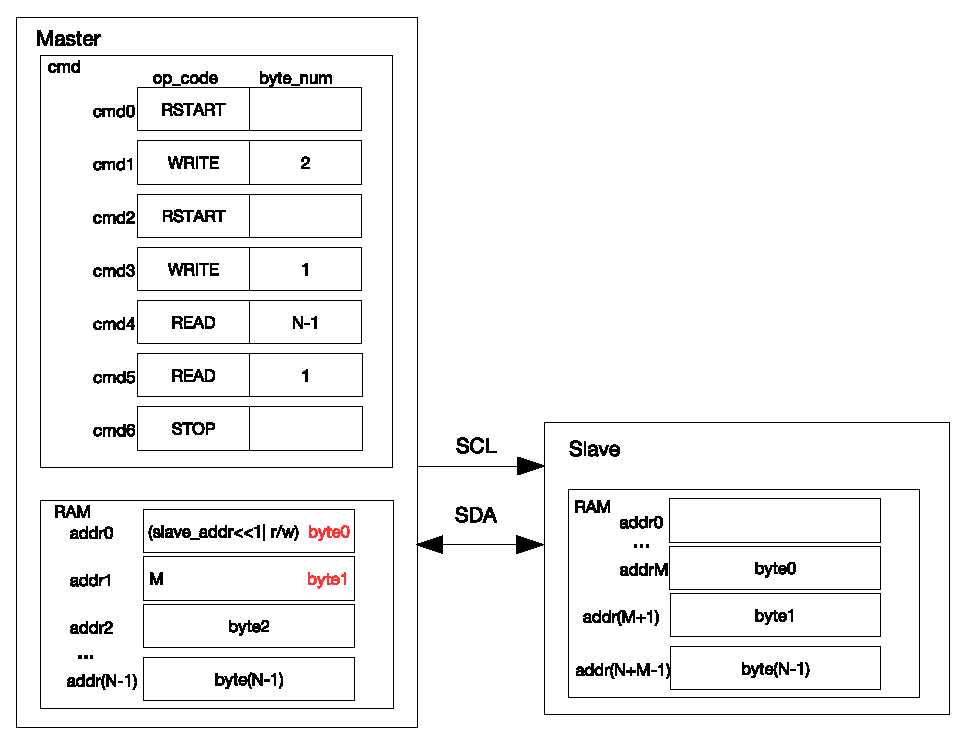
\includegraphics[width=0.8\textwidth]{\modulefiles/figures/I2C_MRS7_M}
    \caption{I2C$_\text{master}$ Reading N Bytes of Data from addrM of I2C$_\text{slave}$ with a 7-bit Address}
    \label{fig:i2c-mrs7-m}
\end{figure}

Figure \ref{fig:i2c-mrs7-m} shows how I2C$_\text{master}$ reads data from specified addresses in an I2C slave. I2C$_\text{master}$ sends two bytes of addresses: the first byte is a 7-bit I2C$_\text{slave}$ address followed by a $R/\overline W$ bit, which is 0 and indicates a WRITE; the second byte is I2C$_\text{slave}$'s memory address. After a RSTART condition, I2C$_\text{master}$ sends the first byte of address again, but the $R/\overline W$ bit is 1 which indicates a READ. Then, I2C$_\text{master}$ reads data starting from addrM.

\subsubsection{Configuration Example}
\begin{enumerate}
\item Set \hyperref[fielddesc:I2CMSMODE]{I2C\_MS\_MODE} (master) to 1, and \hyperref[fielddesc:I2CMSMODE]{I2C\_MS\_MODE} (slave) to 0.
\item We recommend setting \hyperref[fielddesc:I2CSLAVESCLSTRETCHEN]{I2C\_SLAVE\_SCL\_STRETCH\_EN} (slave) to 1, so that SCL can be held low for more processing time when I2C$_\text{slave}$ needs to send data. If this bit is not set, software should write data to be sent to I2C$_\text{slave}$'s TX RAM before I2C$_\text{master}$ initiates transfer. Configuration below is applicable to scenario where \hyperref[fielddesc:I2CSLAVESCLSTRETCHEN]{I2C\_SLAVE\_SCL\_STRETCH\_EN} (slave) is 1.
\item  Set \hyperref[fielddesc:I2CFIFOADDRCFGEN]{I2C\_FIFO\_ADDR\_CFG\_EN} (slave) to 1 to enable double addressing mode.
\item Write 1 to \hyperref[fielddesc:I2CCONFUPGATE]{I2C\_CONF\_UPGATE} (master) and \hyperref[fielddesc:I2CCONFUPGATE]{I2C\_CONF\_UPGATE} (slave) to synchronize registers.
\item Configure command registers of I2C$_\text{master}$.
\begin{longtable}{ | p{4cm} | p{2cm} | p{2cm} | p{2cm} |p{2cm} | p{2cm} |}
\hline\rowcolor{lightgray}
Command registers of I2C$_\text{master}$& op\_code & ack\_value&ack\_exp&ack\_check\_en&byte\_num  \\ \hline
\hyperref[fielddesc:I2CCOMMAND0]{I2C\_COMMAND0} (master)& RSTART& ---&---&---&---  \\ \hline
\hyperref[fielddesc:I2CCOMMAND1]{I2C\_COMMAND1} (master)& WRITE& 0&0&1&2  \\ \hline
\hyperref[fielddesc:I2CCOMMAND2]{I2C\_COMMAND2} (master)& RSTART& ---&---&---&---  \\ \hline
\hyperref[fielddesc:I2CCOMMAND3]{I2C\_COMMAND3} (master)& WRITE& 0&0&1&1  \\ \hline
\hyperref[fielddesc:I2CCOMMAND4]{I2C\_COMMAND4} (master)& READ& 0&0&1&N-1  \\ \hline
\hyperref[fielddesc:I2CCOMMAND5]{I2C\_COMMAND5} (master)& READ& 1&0&1&1  \\ \hline
\hyperref[fielddesc:I2CCOMMAND6]{I2C\_COMMAND6} (master)& STOP& ---&---&---&---  \\ \hline
\end{longtable}

\item Configure \hyperref[fielddesc:I2CSLAVEADDR]{I2C\_SLAVE\_ADDR} (slave) in \hyperref[regdesc:I2CSLAVEADDRREG]{I2C\_SLAVE\_ADDR\_REG} (slave) register as I2C$_\text{slave}$'s 7-bit address, and set \hyperref[fielddesc:I2CADDR10BITEN]{I2C\_ADDR\_10BIT\_EN} (slave) to 0 to enable 7-bit addressing.
\item Write the address of I2C$_\text{slave}$ and data to be sent to TX RAM of I2C$_\text{master}$ in either FIFO or non-FIFO mode according to Section \ref{subsubsec:i2c-txrx}. The first byte of address comprises ( \hyperref[fielddesc:I2CSLAVEADDR]{I2C\_SLAVE\_ADDR}[6:0])<<1) and a $R/\overline W$ bit, which is 0 and indicates a WRITE. The second byte of address is memory address M of I2C$_\text{slave}$. The third byte is ( \hyperref[fielddesc:I2CSLAVEADDR]{I2C\_SLAVE\_ADDR}[6:0])<<1) and a $R/\overline W$ bit, which is 1 and indicates a READ.

\item Write 1 to \hyperref[fielddesc:I2CCONFUPGATE]{I2C\_CONF\_UPGATE} (master) and \hyperref[fielddesc:I2CCONFUPGATE]{I2C\_CONF\_UPGATE} (slave) to synchronize registers.
\item Write 1 to \hyperref[fielddesc:I2CTRANSSTART]{I2C\_TRANS\_START} (master) to start I2C$_\text{master}$'s transfer.
\item Start I2C$_\text{slave}$'s transfer according to Section \ref{subsubsec:i2c-start}.
\item I2C$_\text{slave}$ compares the slave address sent by I2C$_\text{master}$ with its own address in \hyperref[fielddesc:I2CSLAVEADDR]{I2C\_SLAVE\_ADDR} (slave). When ack\_check\_en (master) in I2C$_\text{master}$'s WRITE command is 1, I2C$_\text{master}$ checks ACK value each time it sends a byte. When ack\_check\_en (master) is 0, I2C$_\text{master}$ does not check ACK value and take I2C$_\text{slave}$ as matching slave by default.
\begin{itemize}
\item Match: If the received ACK value matches ack\_exp (master) (the expected ACK value), I2C$_\text{master}$ continues data transfer.
\item Not match: If the received ACK value does not match ack\_exp, I2C$_\text{master}$ generates an I2C\_NACK\_INT (master) interrupt and stops data transfer.
\end{itemize}
\item I2C$_\text{slave}$ receives memory address sent by I2C$_\text{master}$ and adds the offset.
\item I2C$_\text{master}$ sends a RSTART and the third byte in TX RAM, which is ((0x{}78 | \hyperref[fielddesc:I2CSLAVEADDR]{I2C\_SLAVE\_ADDR}[9:8])<<1) and a R bit.
\item I2C$_\text{slave}$ repeats step 11. If its address matches the address sent by I2C$_\text{master}$, I2C$_\text{slave}$ proceed on to the next steps.

\item After \hyperref[int:i2c-slave-stretch]{I2C\_SLAVE\_STRETCH\_INT} (slave) is generated, the \hyperref[fielddesc:I2CSTRETCHCAUSE]{I2C\_STRETCH\_CAUSE} bit is 0. The address of I2C$_\text{slave}$ matches the address sent over SDA, and I2C$_\text{slave}$ needs to send data.

\item Write data to be sent to TX RAM of I2C$_\text{slave}$ in either FIFO mode or non-FIFO mode according to Section \ref{subsubsec:i2c-txrx}.
\item Set \hyperref[fielddesc:I2CSLAVESCLSTRETCHCLR]{I2C\_SLAVE\_SCL\_STRETCH\_CLR} (slave) to 1 to release SCL.


\item I2C$_\text{slave}$ sends data, and I2C$_\text{master}$ checks ACK value or not according to ack\_check\_en (master) in the READ command.
\item If data to be read by I2C$_\text{master}$ is larger than 32 bytes, an \hyperref[int:i2c-slave-stretch]{I2C\_SLAVE\_STRETCH\_INT} (slave) interrupt will be generated when TX RAM of I2C$_\text{slave}$ becomes empty. In this way, I2C$_\text{slave}$ can hold SCL low, so that software has more time to pad data in TX RAM of I2C$_\text{slave}$ and read data in RX RAM of I2C$_\text{master}$. After software has finished reading, you can set \hyperref[fielddesc:I2CSLAVESTRETCHINTCLR]{I2C\_SLAVE\_STRETCH\_INT\_CLR} (slave) to 1 to clear interrupt, and set \hyperref[fielddesc:I2CSLAVESCLSTRETCHCLR]{I2C\_SLAVE\_SCL\_STRETCH\_CLR} (slave) to release the SCL line.

\item After I2C$_\text{master}$ has received the last byte of data, set ack\_value (master) to 1. I2C$_\text{slave}$ will stop transfer once receiving the I2C\_NACK\_INT interrupt.

\item After data transfer completes, I2C$_\text{master}$ executes the STOP command, and generates an I2C\_TRANS\_COMPLETE\_INT (master) interrupt.
\end{enumerate}


\subsection{\texorpdfstring{I2C$_\text{master}$ Reads I2C$_\text{slave}$ with a 7-bit Address in Multiple Command Sequences}{I2C master Reads I2C slave with a 7-bit Address in Multiple Command Sequences}}
\subsubsection{Introduction}
\begin{figure}[H]
    \centering
    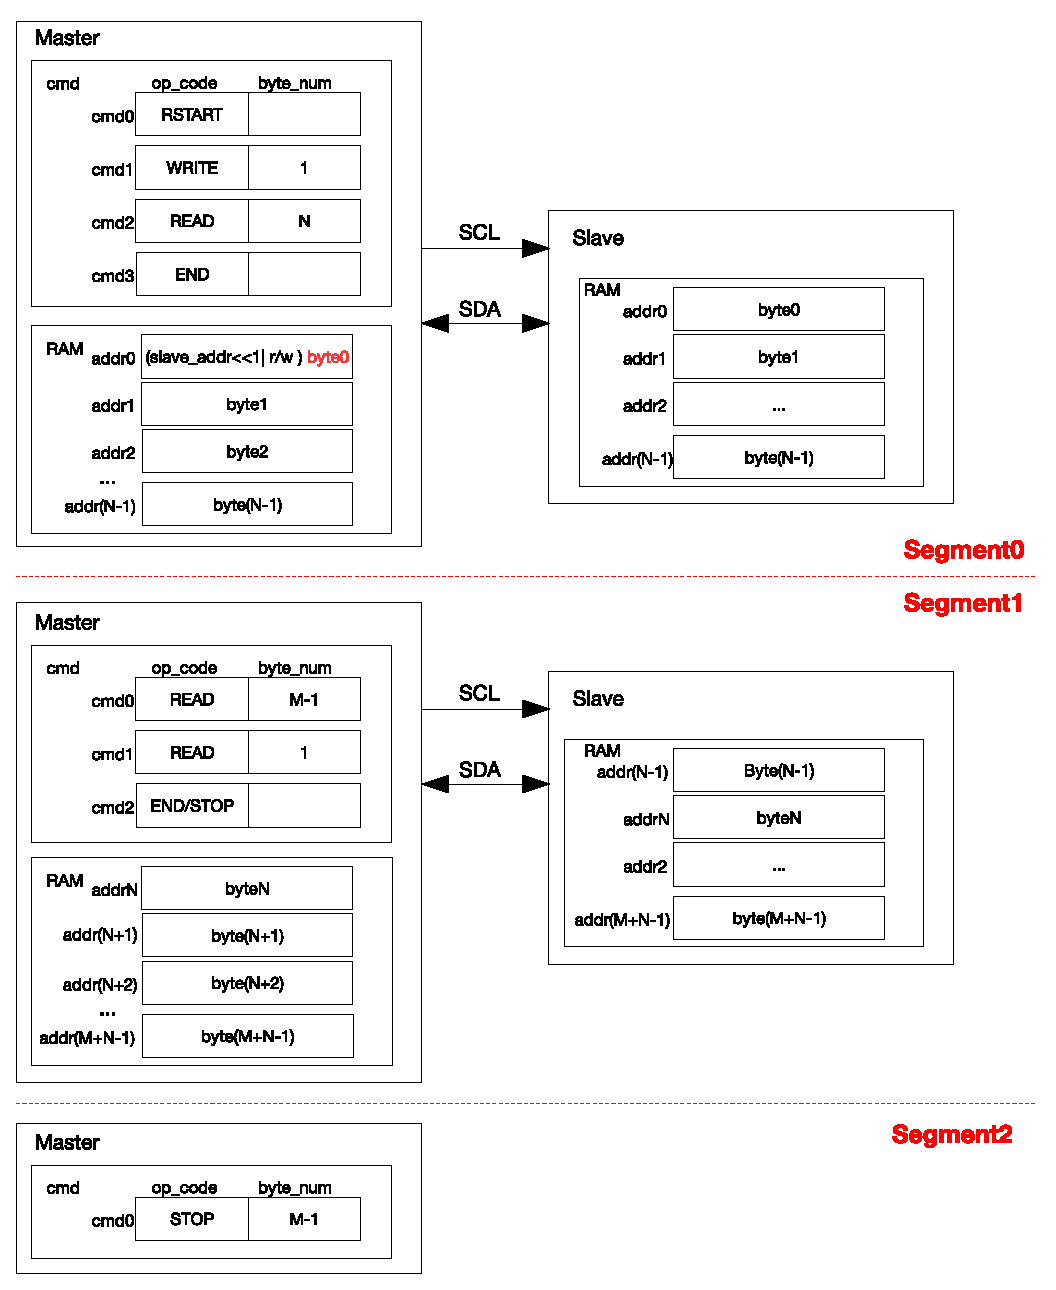
\includegraphics[width=0.8\textwidth]{\modulefiles/figures/I2C_MRS_END}
    \caption{I2C$_\text{master}$ Reading I2C$_\text{slave}$ with a 7-bit Address in Segments}
    \label{fig:i2c-mrs7-multiple}
\end{figure}

Figure \ref{fig:i2c-mrs7-multiple}  shows how I2C$_\text{master}$ reads (N+M) bytes of data from an I2C slave in two/three segments separated by END commands. Configuration procedures are described as follows:
\begin{enumerate}
    \item The procedures for Segment0 is similar to \ref{fig:i2c-mrs7}, except that the last command is an END.
    \item Prepare data in the TX RAM of I2C$_\text{slave}$, and set \hyperref[fielddesc:I2CTRANSSTART]{I2C\_TRANS\_START} to start data transfer. After executing the END command, I2C$_\text{master}$ refreshes command registers and the RAM as shown in Segment1, and clears the corresponding I2C\_END\_DETECT\_INT interrupt. If cmd2 in Segment1 is a STOP, then data is read from I2C$_\text{slave}$ in two segments. I2C$_\text{master}$ resumes data transfer by setting \hyperref[fielddesc:I2CTRANSSTART]{I2C\_TRANS\_START} and terminates the transfer by sending a STOP bit.
    \item If cmd2 in Segment1 is an END, then data is read from I2C$_\text{slave}$ in three segments. After the second data transfer finishes and an I2C\_END\_DETECT\_INT interrupt is detected, the cmd box is configured as shown in Segment2. Once \hyperref[fielddesc:I2CTRANSSTART]{I2C\_TRANS\_START} is set, I2C$_\text{master}$ terminates the transfer by sending a STOP bit.

\end{enumerate}

\subsubsection{Configuration Example}
\begin{enumerate}
\item Set \hyperref[fielddesc:I2CMSMODE]{I2C\_MS\_MODE} (master) to 1, and \hyperref[fielddesc:I2CMSMODE]{I2C\_MS\_MODE} (slave) to 0.
\item We recommend setting \hyperref[fielddesc:I2CSLAVESCLSTRETCHEN]{I2C\_SLAVE\_SCL\_STRETCH\_EN} (slave) to 1, so that SCL can be held low for more processing time when I2C$_\text{slave}$ needs to send data. If this bit is not set, software should write data to be sent to I2C$_\text{slave}$'s TX RAM before I2C$_\text{master}$ initiates transfer. Configuration below is applicable to scenario where \hyperref[fielddesc:I2CSLAVESCLSTRETCHEN]{I2C\_SLAVE\_SCL\_STRETCH\_EN} (slave) is 1.
\item Write 1 to \hyperref[fielddesc:I2CCONFUPGATE]{I2C\_CONF\_UPGATE} (master) and \hyperref[fielddesc:I2CCONFUPGATE]{I2C\_CONF\_UPGATE} (slave) to synchronize registers.
\item Configure command registers of I2C$_\text{master}$.
\begin{longtable}{ | p{4cm} | p{2cm} | p{2cm} | p{2cm} |p{2cm} | p{2cm} |}
\hline\rowcolor{lightgray}
Command registers of I2C$_\text{master}$& op\_code & ack\_value&ack\_exp&ack\_check\_en&byte\_num  \\ \hline
\hyperref[fielddesc:I2CCOMMAND0]{I2C\_COMMAND0} (master)& RSTART& ---&---&---&---  \\ \hline
\hyperref[fielddesc:I2CCOMMAND1]{I2C\_COMMAND1} (master)& WRITE& 0&0&1&1  \\ \hline
\hyperref[fielddesc:I2CCOMMAND2]{I2C\_COMMAND2} (master)& READ& 0&0&1&N  \\ \hline
\hyperref[fielddesc:I2CCOMMAND3]{I2C\_COMMAND3} (master)& END& ---&---&---&---  \\ \hline
\end{longtable}
\item Write the address of I2C$_\text{slave}$ to TX RAM of I2C$_\text{master}$ in FIFO or non-FIFO mode.
\item Write the address of I2C$_\text{slave}$ to \hyperref[fielddesc:I2CSLAVEADDR]{I2C\_SLAVE\_ADDR} (slave) in \hyperref[regdesc:I2CSLAVEADDRREG]{I2C\_SLAVE\_ADDR\_REG} (slave) register.
\item Write 1 to \hyperref[fielddesc:I2CCONFUPGATE]{I2C\_CONF\_UPGATE} (master) and \hyperref[fielddesc:I2CCONFUPGATE]{I2C\_CONF\_UPGATE} (slave) to synchronize registers.
\item Write 1 to \hyperref[fielddesc:I2CTRANSSTART]{I2C\_TRANS\_START} (master) to start I2C$_\text{master}$'s transfer.
\item Start I2C$_\text{slave}$'s transfer according to Section \ref{subsubsec:i2c-start}.
\item I2C$_\text{slave}$ compares the slave address sent by I2C$_\text{master}$ with its own address in \hyperref[fielddesc:I2CSLAVEADDR]{I2C\_SLAVE\_ADDR} (slave). When ack\_check\_en (master) in I2C$_\text{master}$'s WRITE command is 1, I2C$_\text{master}$ checks ACK value each time it sends a byte. When ack\_check\_en (master) is 0, I2C$_\text{master}$ does not check ACK value and take I2C$_\text{slave}$ as matching slave by default.
\begin{itemize}
\item Match: If the received ACK value matches ack\_exp (master) (the expected ACK value), I2C$_\text{master}$ continues data transfer.
\item Not match: If the received ACK value does not match ack\_exp, I2C$_\text{master}$ generates an I2C\_NACK\_INT (master) interrupt and stops data transfer.
\end{itemize}

\item After \hyperref[int:i2c-slave-stretch]{I2C\_SLAVE\_STRETCH\_INT} (slave) is generated, the \hyperref[fielddesc:I2CSTRETCHCAUSE]{I2C\_STRETCH\_CAUSE} bit is 0. The address of I2C$_\text{slave}$ matches the address sent over SDA, and I2C$_\text{slave}$ needs to send data.

\item Write data to be sent to TX RAM of I2C$_\text{slave}$ in either FIFO mode or non-FIFO mode according to Section \ref{subsubsec:i2c-txrx}.
\item Set \hyperref[fielddesc:I2CSLAVESCLSTRETCHCLR]{I2C\_SLAVE\_SCL\_STRETCH\_CLR} (slave) to 1 to release SCL.


\item I2C$_\text{slave}$ sends data, and I2C$_\text{master}$ checks ACK value or not according to ack\_check\_en (master) in the READ command.
\item If data to be read by I2C$_\text{master}$ in one READ command (N or M) is larger than 32 bytes, an \hyperref[int:i2c-slave-stretch]{I2C\_SLAVE\_STRETCH\_INT} (slave) interrupt will be generated when TX RAM of I2C$_\text{slave}$ becomes empty. In this way, I2C$_\text{slave}$ can hold SCL low, so that software has more time to pad data in TX RAM of I2C$_\text{slave}$ and read data in RX RAM of I2C$_\text{master}$. After software has finished reading, you can set \hyperref[fielddesc:I2CSLAVESTRETCHINTCLR]{I2C\_SLAVE\_STRETCH\_INT\_CLR} (slave) to 1 to clear interrupt, and set \hyperref[fielddesc:I2CSLAVESCLSTRETCHCLR]{I2C\_SLAVE\_SCL\_STRETCH\_CLR} (slave) to release the SCL line.
\item Once finishing reading data in the first READ command, I2C$_\text{master}$ executes the END command and triggers an I2C\_END\_DETECT\_INT (master) interrupt, which is cleared by setting \hyperref[fielddesc:I2CENDDETECTINTCLR]{I2C\_END\_DETECT\_INT\_CLR} (master) to 1.
\item Update I2C$_\text{master}$'s command registers using one of the following two methods:
\begin{longtable}{ | p{4cm} | p{2cm} | p{2cm} | p{2cm} |p{2cm} | p{2cm} |}
\hline\rowcolor{lightgray}
Command registers of I2C$_\text{master}$& op\_code & ack\_value&ack\_exp&ack\_check\_en&byte\_num  \\ \hline
\hyperref[fielddesc:I2CCOMMAND0]{I2C\_COMMAND0} (master)& READ& ack\_value&ack\_exp&1&M  \\ \hline
\hyperref[fielddesc:I2CCOMMAND1]{I2C\_COMMAND1} (master)& END& ---&---&---&---  \\ \hline
\end{longtable}
Or
\begin{longtable}{ | p{4cm} | p{2cm} | p{2cm} | p{2cm} |p{2cm} | p{2cm} |}
\hline\rowcolor{lightgray}
Command registers of I2C$_\text{master}$& op\_code & ack\_value&ack\_exp&ack\_check\_en&byte\_num  \\ \hline
\hyperref[fielddesc:I2CCOMMAND0]{I2C\_COMMAND0} (master)& READ& 0&0&1&M-1  \\ \hline
\hyperref[fielddesc:I2CCOMMAND0]{I2C\_COMMAND0} (master)& READ& 1&0&1&1  \\ \hline
\hyperref[fielddesc:I2CCOMMAND1]{I2C\_COMMAND1} (master)& STOP& ---&---&---&---  \\ \hline
\end{longtable}

\item Write M bytes of data to be sent to TX RAM of I2C$_\text{slave}$. If M is larger than 32, then repeat step 14 in FIFO or non-FIFO mode.
\item Write 1 to \hyperref[fielddesc:I2CTRANSSTART]{I2C\_TRANS\_START} (master) bit to start transfer and repeat step 14.
\item If the last command is a STOP, then set ack\_value (master) to 1 after I2C$_\text{master}$ has received the last byte of data. I2C$_\text{slave}$ stops transfer upon the I2C\_NACK\_INT interrupt. I2C$_\text{master}$ executes the STOP command to stop transfer and generates an I2C\_TRANS\_COMPLETE\_INT (master) interrupt.
\item If the last command is an END, then repeat step 16 and proceed on to the next steps.
\item Update I2C$_\text{master}$'s command registers.
\begin{longtable}{ | p{4cm} | p{2cm} | p{2cm} | p{2cm} |p{2cm} | p{2cm} |}
\hline\rowcolor{lightgray}
Command registers of I2C$_\text{master}$& op\_code & ack\_value&ack\_exp&ack\_check\_en&byte\_num  \\ \hline
\hyperref[fielddesc:I2CCOMMAND1]{I2C\_COMMAND1} (master)& STOP& ---&---&---&---  \\ \hline
\end{longtable}
\item Write 1 to \hyperref[fielddesc:I2CTRANSSTART]{I2C\_TRANS\_START} (master) bit to start transfer.
\item I2C$_\text{master}$ executes the STOP command to stop transfer, and generates an I2C\_TRANS\_COMPLETE\_INT (master) interrupt.

\end{enumerate}

\section{Interrupts}\label{sub:i2c-int}
\begin{itemize}
\item \label{int:i2c-slave-stretch}I2C\_SLAVE\_STRETCH\_INT: Generated when one of the four stretching events occurs in slave mode.
\item \label{int:i2c-start}I2C\_DET\_START\_INT: Triggered when the master or the slave detects a START bit.
\item \label{int:i2c-scl-main-fsm}I2C\_SCL\_MAIN\_ST\_TO\_INT: Triggered when the main state machine SCL\_MAIN\_FSM remains unchanged for over \hyperref[fielddesc:I2CSCLMAINSTTOI2C]{I2C\_SCL\_MAIN\_ST\_TO\_I2C}[23:0] clock cycles.
\item \label{int:i2c-scl-fsm}I2C\_SCL\_ST\_TO\_INT: Triggered when the state machine SCL\_FSM remains unchanged for over \\\hyperref[fielddesc:I2CSCLSTTOI2C]{I2C\_SCL\_ST\_TO\_I2C}[23:0] clock cycles.
\item \label{int:i2c-rxfifo-udf}I2C\_RXFIFO\_UDF\_INT: Triggered when the I2C controller reads RX FIFO via the APB bus, but RX FIFO is empty.
\item \label{int:i2c-txfifo-ovf}I2C\_TXFIFO\_OVF\_INT: Triggered when the I2C controller writes TX FIFO via the APB bus, but TX FIFO is full.
\item \label{int:i2c-nack}I2C\_NACK\_INT: Triggered when the ACK value received by the master is not as expected, or when the ACK value received by the slave is 1.
\item \label{int:i2c-trans-start}I2C\_TRANS\_START\_INT: Triggered when the I2C controller sends a START bit.
\item \label{int:i2c-time-out}I2C\_TIME\_OUT\_INT: Triggered when SCL stays high or low for more than 2$^{\hyperref[fielddesc:I2CTIMEOUTVALUE]{I2C\_TIME\_OUT\_VALUE}}$ clock cycles during data transfer.
\item \label{int:i2c-trans-complete}I2C\_TRANS\_COMPLETE\_INT: Triggered when the I2C controller detects a STOP bit.
\item \label{int:i2c-mst-txfifo-udf}I2C\_MST\_TXFIFO\_UDF\_INT: Triggered when TX FIFO of the master underflows.
\item \label{int:i2c-arbitration-lost}I2C\_ARBITRATION\_LOST\_INT: Triggered when the SDA's output value does not match its input value while the master's SCL is high.
\item \label{int:i2c-byte-trans-done}I2C\_BYTE\_TRANS\_DONE\_INT: Triggered when the I2C controller sends or receives a byte.
\item \label{int:i2c-end}I2C\_END\_DETECT\_INT: Triggered when op\_code of the master indicates an END command and an END condition is detected.
\item \label{int:i2c-rxfifo-ovf}I2C\_RXFIFO\_OVF\_INT: Triggered when RX FIFO of the I2C controller overflows.
\item \label{int:i2c-txfifo-wm}I2C\_TXFIFO\_WM\_INT: I2C TX FIFO watermark interrupt. Triggered when \hyperref[fielddesc:I2CFIFOPRTEN]{I2C\_FIFO\_PRT\_EN} is 1 and the pointers of TX FIFO are less than \hyperref[fielddesc:I2CTXFIFOWMTHRHD]{I2C\_TXFIFO\_WM\_THRHD}[4:0].
\item \label{int:i2c-rxfifo-wm}I2C\_RXFIFO\_WM\_INT: I2C RX FIFO watermark interrupt. Triggered when \hyperref[fielddesc:I2CFIFOPRTEN]{I2C\_FIFO\_PRT\_EN} is 1 and the pointers of RX FIFO are greater than \hyperref[fielddesc:I2CRXFIFOWMTHRHD]{I2C\_RXFIFO\_WM\_THRHD}[4:0].
\end{itemize}


% >>> If your module has no registers, delete sample text
%       for Sections Register Summary and Registers below <<<

%%%%%%%%%%%%%%%%%%%%%%%%
%%% Register Summary %%%
%%%%%%%%%%%%%%%%%%%%%%%%

% >>> Update the sample text below and insert
%     the info on register summary into the subfile <<<

\clearpage
\section{Register Summary}
\label{sec:i2c-reg-summ}
\hypertarget{i2c-reg-summ}{}

The addresses in this section are relative to \textcolor{red}{I2C Controller} base address provided in Table \ref{tab:sysmem-base-address} in Chapter \ref{mod:sysmem} \textit{\nameref{mod:sysmem}}.

The abbreviations given in Column \textbf{Access} are explained in Section \hyperref[glossary-access-types]{\textit{Access Types for Registers}}.

\subfile{\modulefiles/01-I2C-reg-summ__EN}


%%%%%%%%%%%%%%%%%
%%% Registers %%%
%%%%%%%%%%%%%%%%%

% >>> Update the sample text below and insert
%      the info on registers into the subfile <<<

\clearpage
\section{Registers}

The addresses in this section are relative to \textcolor{red}{I2C Controller} base address provided in Table \ref{tab:sysmem-base-address} in Chapter \ref{mod:sysmem} \textit{\nameref{mod:sysmem}}.

\subfile{\modulefiles/01-I2C-reg__EN}


\end{document}
